\documentclass[pageno]{jpaper}

%replace XXX with the submission number you are given from the ASPLOS submission site.
\newcommand{\asplossubmissionnumber}{XXX}

\usepackage[normalem]{ulem}
\usepackage{graphicx}
\usepackage{amsmath}
\usepackage{xcolor}
\usepackage{fancyhdr}
\usepackage{hyperref}
\usepackage{bbm}
\usepackage{times}
\usepackage{soul}
\usepackage[utf8]{inputenc}
\usepackage{latexsym}
\usepackage{amsmath}
\usepackage{graphicx}
\usepackage{caption}
\usepackage{subcaption}
\usepackage{amssymb}


%\usepackage[colorinlistoftodos]{todonotes}
\usepackage{algorithm}
\usepackage{algpseudocode}
%\graphicspath{ {images/} }
%\usepackage[square,sort,comma,numbers]{natbib}

\usepackage{float}
\floatstyle{plaintop}
\restylefloat{table}

\usepackage{graphicx,epstopdf}
\epstopdfsetup{update}
\DeclareGraphicsExtensions{.ps}
\epstopdfDeclareGraphicsRule{.ps}{pdf}{.pdf}{ps2pdf -dEPSCrop -dNOSAFER #1 \OutputFile}




\begin{document}

\title{SECS: Efficient Deep Stream Processing via Class Skew Dichotomy}
\author{}
\date{}
\maketitle

%\thispagestyle{empty}

\begin{abstract}
As accelerating CNNs receives an increasing research focus, the save in resource always comes with a decrease in accuracy. To both increase accuracy and decrease resource consumption, we explore an environment information, called \textit{class skew}, which is easily available and exists widely in day-to-day life. Since the class skew may switch as time goes, we bring up \textit{probability layer} to utilize class skew without any overhead during the runtime. Further, we observe \textit{class skew dichotomy} that some class skew may appear frequently in the future, called \textit{hot class skew} and others will never appear again, called \textit{cold class skew}. Inspired by techniques from source code optimization, two modes, i.e., interpretation and compilation, are proposed. The interpretation mode pursues efficient adaption during runtime for cold class skew and the compilation mode aggressively optimize on hot ones for more efficient deployment in the future. Aggressive optimization is processed by class-specific pruning and provides extra benefit. Finally, we design a systematic framework, SECS, to dynamically detect class skew, processing interpretation and compilation, as well as select the most accurate architectures under the runtime resource budget. Evaluations on recognizing faces in TV shows and movies show that SECS can realize end-to-end classification speedups of xxx/xxx (on GPU/CPU) relative to a state-of-the-art convolutional neural network, at competitive accuracy.
\end{abstract}




\section{Introduction}
Modern convolutional neural networks (CNNs) has made unprecedented advance in visual recognition tasks. In 2012, AlexNet \cite{krizhevsky2012imagenet} achieved a top-5 error of 17\% on ImageNet \cite{deng2009imagenet}, while previous method could only achieve a top-5 error of 25.7\%. Since then, CNNs have become the dominant method and main research direction in image recognition. In 2015, ResNet \cite{he2016deep} achieved a top-5 error of 3.57\%, supressing the human-level classification error rate on ImageNet reported as 5.1\% \cite{russakovsky2015imagenet}. The success of CNNs on visual recognition tasks has fueled the desire to deploy these networks on various kind of mobile platforms and has an increasingly important role in daily life, e.g., in robotics, self-driving cars, and on cell phones. These applications are usually computation-intensive and latency-sensitive, while running on resource-constrained devices. 

To enable the deployment of CNNs on mobile platforms, an increasing research focus has been received by accelerating CNNs, basically trading accuracy for less resource consumption. One approach is to prune the model utilizing the spatial redundancy inside the architecture. LCNN \cite{bagherinezhad2017lcnn} utilizes network quantization to achieve a $5$x speedup at a loss of $7.1$\% accuracy for the ResNet-18 model \cite{he2016deep}. On VGG-16 \cite{simonyan2014very}, filter pruning \cite{lin2018accelerating} is used to reduce computation by $4$x while the accuracy is also decreased by $2.81$\%. Another approach is to build a model store and dynamically select the most accurate model under available resource budget during runtime. 
While these pruning methods and scheduling models can reduce the resource consumption, a decrease in accuracy is also introduced, which is not desired.







While the deployment on these platforms shows an inspiring perspective, the nature of limited resource on these platforms still obstacles the accessibility of CNNs. For example, large data transfer is required while over-the-air updates has been reported to incrementally improve the safety of Tesla's Autopilot semi-autonomous driving functionality \cite{teslas2018}. With AlexNet\cite{krizhevsky2012imagenet} and VggNet \cite{simonyan2014very}, more than 60MB and 138MB parameters need to be transferred from the server to the car respectively. To make the model updating more feasible, smaller models with less parameters are preferred. Another challenge for the deployment is the intensive computation of CNNs. Tens of GFLOPs computation is needed by modern CNNs for processing a single image \cite{canziani2016analysis}. While multiple GPUs can be grouped together to train and process images in lab, the intensive computation consumed by modern CNNs are not affordable for most mobile platforms. Thus, to better fulfill the requirement of limited resource, CNNs need to be resource-aware and the architectures need to be adjusted according to the available resource budget, i.e., energy and memory.

We observe that the input data to mobile platforms in the real world usually has strong temporal correlation. While thousands of objects may appear in our daily life, only a small portion of objects can be seen in most specific scenarios, called \textit{runtime class skew}. For example, we may meet thousands of people through the whole year, but only less than ten people could appear in our lab. Actually, experiments on videos of day-to-day life \cite{shen2016fast} shows that $10$ objects comprised $90$\% of all objects in $85$\% time. To meet the requirement of classifying these $10$ objects, a small model with $10$ classes with less than $10$ classes would be sufficient and the huge model classifying thousands of objects could be escaped. 

While recent works involve utilizing runtime class skew, we provide an efficient way to adapt the model according to runtime information. Specifically, all of existing works \cite{han2016mcdnn, shen2016fast} require runtime finetuning, which uses transfer learning \cite{doersch2015unsupervised, noroozi2016unsupervised, oquab2014learning, yosinski2014transferable} to adapt the last few layers towards the runtime class skew. MCDNN \cite{han2016mcdnn} flows all training inputs through lower layers at compile time to avoid parts of computation during runtime. Even if pre-computation is deployed, a 14-second latency still exist, which obstacle the feasibility of utilizing runtime class skew. In contrast, we take an unusual approach, called \textit{probability layer}, to utilize runtime class skew without any finetuning and achieve an euqal or better performance.

Once utilizing runtime class skew has increased accuracy dramatically, new chance appears for using more aggressive pruning methods. In fact, the main drawback of current pruning methods is the reduction in accuracy. The standard approaches involve matrix factorization \cite{jaderberg2014speeding, kim2015compression, xue2014singular}, matrix pruning \cite{chen2015compressing, han2015learning}, quantization \cite{bagherinezhad2017lcnn, han2015deep} and group convolution \cite{howard2017mobilenets, ZhaZho17ShuffleNet}. All of these methods prune an architecture with given hyper-parameters, i.e. number of layers, channel connections, and number of neurons. When hyper-parameters become the pruning target, hand-crafted architectures are still used and trail-and-errors is the only approach to compare different architectures. Selecting hyper-parameters is challenging since we cannot know the accuracy of the new architecture before it is actually trained and tested. Considering that modern CNNs usually takes days or even weeks to train, only a limited number of hyper-parameters could be used, which limits the exploration space dramtically.

Instead, we observe that CNNs often have strong redundancy inside its structure, i.e., within feature maps, across channels, and across layers. Inspired by the loop perforation technique from source code optimization \cite{figurnov2016perforatedcnns}, we can speed up computation by skipping their evaluation in some of the positions. We further observe that different positions has different redundancy and we can select the hyper-parameter according to their influence over final accuracy. Based on these insight, we propose a framework, called \textit{perforation}, for selecting hyper-parameters in three levels; i.e., neuron-wise, channel-wise, and layer-wise, without any finetune for the new architecture and agnostic to the model architecture. While carefully hand-crafted architecture, SqueezeNet, achieves AlexNet-level accuracy with $50$x less parameters, perforation can reach $600$x reduction in parameters while also achieve AlexNet-level accuracy. Perforation is orthogonal to matrix factorization, matrix pruning, quantization, and group convolution, and can be combined with all for further optimization. When combined with runtime class skew, perforation can prune the model according to which classes appear in current environment and only maintain the important path for appearing classes.

In this paper, we present \textbf{SECS}, a real-time image classification framework to achieve the above goal.SECS essentially detects and utilize runtime class skew and prune the candidate model according to the environment and the resource budget, as detailed in Section 3. Inspired by the interpretation and compilation in modern programming language, we also propose the two mode for $SECS$. When we first confront a class skew, we utilize probability layer to adapt to runtime class skew without any overhead and only utilize existing models, i.e. \textit{interpretation mode}. Once a class skew has appeared for a number of times more than the pre-defined threshold, the class skew will be marked as "hot" and pruning towards this specific class skew will be deployed, i.e. \textit{compilation mode}, after the resource constrain on the platform is resolved, i.e. connected to electric and network. In addition, we carefully design a scheduling algorithm based on control theory to select the Pareto-optimal models under the available resource budget. Extensive evaluation shows that our system can potentially reduce the computation by xx times and memory consumption by xx times.

In summary, we make the following contributions:

\begin{enumerate}
  \item We bring up \textit{probability layer}, a technique adapting all models to the runtime class skew without any overhead and achieving equal or better accuracy than finetuning.
  \item We propose a pruning approach, \textit{perforation}, for selecting hyper-parameters in three levels; i.e., neuron-wise, channel-wise, and layer-wise, without any finetune for the new architecture and agnostic to the model architecture. Our pruning approach can prune a model to AlexNet-level accuracy with 300x less parameters automatically, compared with the hand-crafted optimization method, \textit{SqueezeNet}, achieving same accuracy with 60x less parameters.
  \item We build a system, \textit{SECS}, as a background service. Extensive evaluation confirms its benefit is significant. (Experiments results to be added). 
\end{enumerate}







\section{Motivation}
\subsection{Motivating applications}
Among the fastest growing applications, vision-based cognitive assistance applications and robotics visions are two representative categories.

As an example cognitive assistance applications, Aira \cite{aria2018} continuously recognizes surrounding environment and help the blind person with ordinary tasks, i.e. reading a handwritten note, navigating the grocery store, and even to run the Boston Marathon. With the record on runtime class skew that appears frequently, including repeated environment and activity, CNN architectures can be optimized towards a more personal assistance. The automatic pruning methods utilize personal behavior pattern locally and protect user privacy perfectly.

On the other hand, robotic visions such as remote-controlled robotic animals \cite{bbc2018} for search specific animals and documenting secret lives of animals in the wild, teleoperated robots \cite{landmine2018} for detecting and removing landmine in various environment, and rover robot \cite{rover2018} for space exploration. 

\paragraph{Common themes.} Most of these operate in the wild environment maintaining a strong temporal locality. According to a experiments on videos of day-to-day life from Youtube \cite{shen2016fast}, $10$ objects comprised $90$\% of all objects in $85$\% time. The class skew may appear for a small time period, which requires efficient model adaption, the \textit{interpretation mode}. Further, some class skews may appear repeatedly, i.e. in our office and lab, which provides chance for pruning model towards the specific class skew, the \textit{compilation mode}.




\subsection{Opportunities}
The above applications all take input from the life-style environment. Such input exhibits runtime class skew, due to activities of the mobile devices showing strong spatial and temporal locality. 

\paragraph{Temporal correlation.} We can view the input stream as a continual camera feed. In the input stream, every frame differs only slightly from previous frames. Thus, the objects in frames usually keep appearing for a time period before the user moves to another scene. For example, a small group of people will appear frequently in a scenario of films, generally lasting for tens of minutes, and another group of people will not appear until the scenario has changed. The runtime class skew appears frequently and provide chance to simplify CNN models. 

\paragraph{Spatial correlation} It is common for humans to follow along recurrent trajectories, for example, due to their regular social activities or frequenting a favorite park from time to time. Therefore, there is some level of recurrence of the scenes obtained as part of those activities. Through these repeating scenarios, same runtime class skew will also keep appearing, which make it a feasible choice to optimize CNNs towards the specific environment.


Utilizing runtime class skew can both increase accuracy and decrease resource consumption. The intuition comes from utilizing runtime class skew in random guessing. If we randomly guess from $1000$ classes, the accuracy is $0.1\%$, while the accuracy would increase to $10\%$ for randomly guessing from $10$ classes. Even if we have changed nothing in the model architecture, the accuracy would increase naturally by decreasing the number of classes. Our experiments have shown that the top-1 accuracy of a 40-layer DenseNet \cite{huang2017densely} on CIFAR100 \cite{krizhevsky2009learning} would increase to 99\% when we constrain the output space to be $5$ classes, while the top-1 accuracy of the 40-layer DenseNet on $100$ classes is only $73.75$\%. Compared to recent works on increasing accuracy through more complex and deep models and dramtically increased resource consumption, utilizing runtime class skew is almost free since we only need to profile the incoming classes and detect the scenario.

Further, utilizing runtime class skew increases accuracy and provides new chance for using more agressive pruning methods. In fact, the main drawback of current pruning methods \cite{bagherinezhad2017lcnn, figurnov2016perforatedcnns, han2015deep, veniat2017learning, wen2016learning} is the reduction in accuracy. For example, while LCNN \cite{bagherinezhad2017lcnn} can reduce the computation by $37.6$x, the top-1 accuracy will also decrease from $56.6$\% to $44.3$. In contrast, once the runtime class skew is detected, models can be adapted efficiently with probability layer and accuracy can be increased dramatically. Since probability layer is agnostic to model architecture, the Pareto-optimal model under available resource budget can be selected and combined with probability layer directly without any overhead.


\subsection{Common processing steps}


\begin{figure}
  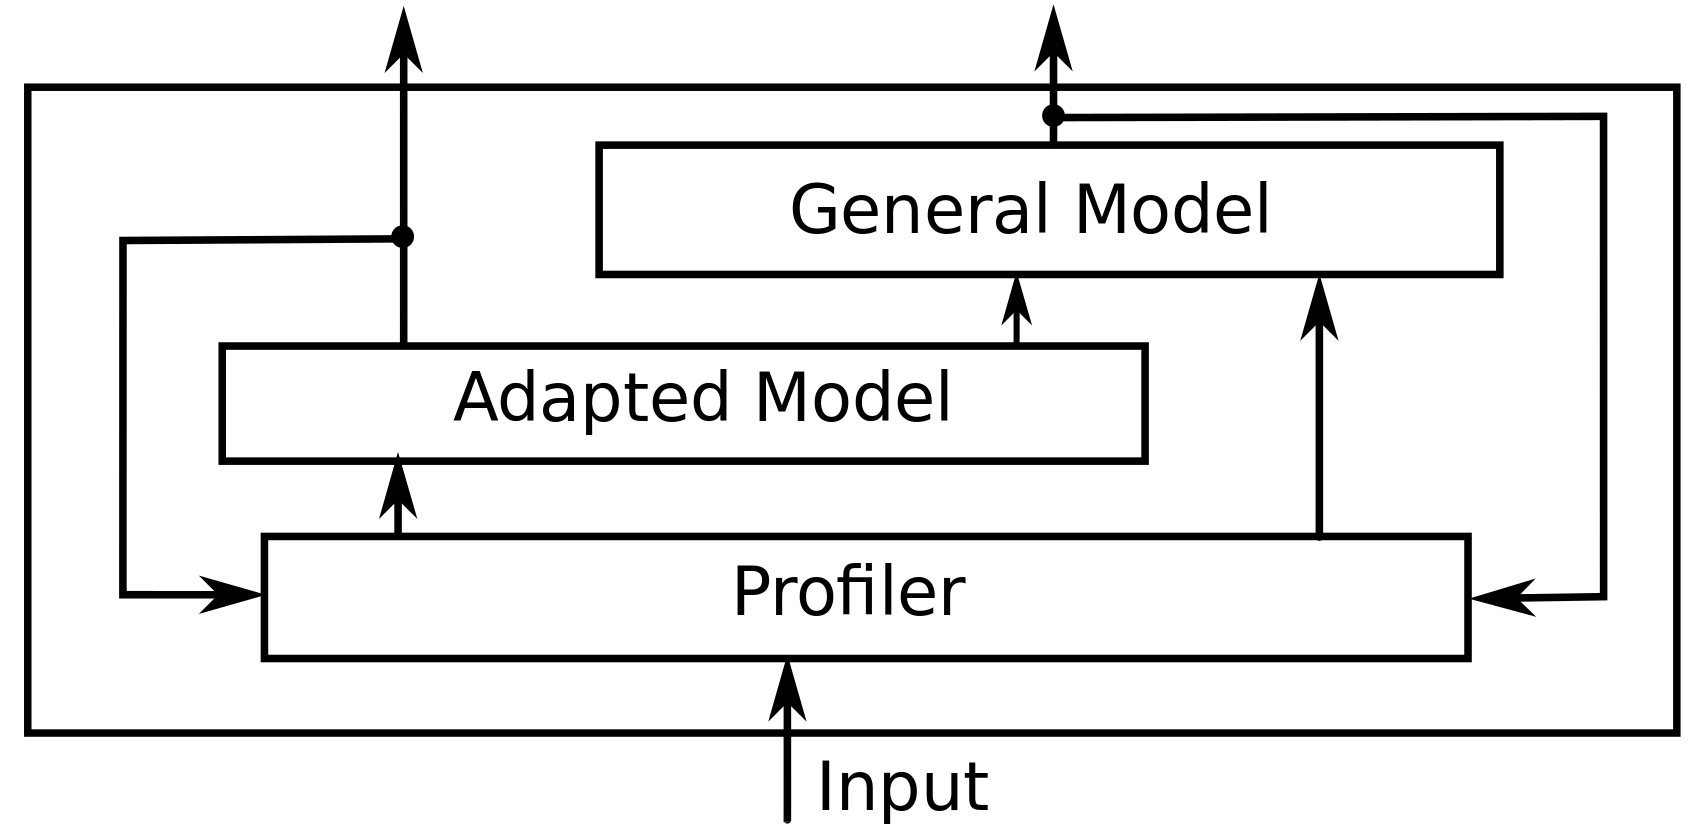
\includegraphics[scale=0.14]{profiler.png}
  \caption{Schematic processing flow.}
  \label{fig:profiler}
\end{figure}

Figure \ref{fig:profiler} shows the schematic processing flow of an input image, as depicted in . When new input comes, the profiler will check whether there is class skew in current environment. If not, the input will be forwarded to a general model handling all possible classes. After the general model classify the input image, results will be both sent to the user and processed profiler to update class distribution. Once the profiler decides that a class skew has appeared, an adapted model will be generated efficiently according to available resource budget and desired accuracy. Then, the input will be forwarded to the adapted model, which consumes less resource, instead of the general model. Once the adapted model has finished the process of image and has strong confident in the results, the result will also be send to the user and used to update the class distribution in profiler. If the adapted model is not confident, the input will be forwarded to the general model and a more accurate procedure will be employed. Entropy and the value of predicted class could be used as a measure of model confidence. After a time period, when the profiler detects a new class skew, i.e. the user arrive at a new place, the model will be adapted towards the new environment and replace the old one. The detection of class skew could be done by profiler according to existing works. 

Existing works must forward the input to the general model for further speculation when the adapted model is not confident, because new classes may have appeared and the adapted model could only detect a small group of classes. Probability layer solved this problem by forcing the model to considering the runtime class skew while still maintain the ability to choose from classes that have never appeared when there is a strong reason to do so. Thus the forwarding of images to general model could be escaped in our design, which reduces lots of overhead.







\subsection{Challenges}
The challenge remains in two respective; i.e. how to utilize runtime class skew efficiently and how to prune the model towards desired resource budget automatically. 

In order to effectively utilize runtime class skew, we need efficient method to adapt the pretrained architecture towards environment, with little or no resource consumption and temporal latency. Intuitively, model adaption, especially when the number of target classes has decreased dramatically, requires changing the architecture, e.g., the reduction on number of nodes in the softmax layer. Recent works finetune the last few layers for adapting the model to runtime class skew. However, finetuning during runtime is unfeasible since it brings tremendous overhead in both computation and memory. It is also infeasible to adapt the pre-trained model to all possible class skews beforehand. Considering the number of combinations, if we take $10$ classes out of $100$ classes, the total count of combinations would achieve a mind-bogglingly huge number of $1.73*10^{14}$. Further, it is also hard to decide number of layers to be finetuned. Recent work \cite{yosinski2014transferable} reports that co-adaption between adjacent layers and spliting networks between co-adapted layers may hurt the performance dramatically. 

Automatic pruning models and selecting hyper-parameters is also challenging. The changed architectures require a long-time training to get the performance, which limits the search space of hyper-parameters dramatically. To generate a cascade of models with different resource consumption and performance, existing papers utilize hand-selected architectures, which is not a automatical procedure and only a small number of hyperparameters can be tested. Specifically, NoScope \cite{kang2017noscope} only performs model search by varying the number of convolutional layers (2 or 4), number of convolution units in the base layer (32 or 64), and number of neurons in the fully connected layer (32, 64, 128, or 256). MCDNN \cite{han2016mcdnn} chooses between reduce number of nodes in fully connected layers, decrease number of kernels, and eliminate convolutional layers entirely. FastVideo \cite{shen2016fast} also manually removes layers, decreases kernel sizes, increases kernel strides, and reduces the size of fully-connected layers, to generate a cascade of models with the tradeoff between accuracy and resource consumption. All these manually selected architectures requires human interfere. Automatic pruning is challenge since once we change the model architecture we cannot precess an image and get the accuracy until the model is trained again. We cannot even get a cascade of models with decreasing accuracy before we train and test the architectures one by one. To make system framework for mobile platforms and model pruning towards runtime class skew more feasible, it is necessary to find an approach pruning models automatically and generate a cascade of models with decreasing accuracy without training.

We address these challenges by probability layer, an efficient model adaption algorithm, and perforation, an automatic pruning methods. Further, we designed a real-time image classification framework, SECS, to automatically detect and utilize runtime class skew and select the Pareto-optimal models under available resource budget.
























\section{SECS System Design}
\subsection{Overview}
SECS utilize runtime class skew efficiently and optimize architectures automatically to provide real-time image classification. When an input comes, it will be processed by a general model and the results will be recorded by the profiler to update the distribution. Once the profiler decides that a runtime class skew has appeared, an adapted model will be generated efficiently by probability layer and future inputs will be handled by the adapted model instead of the general model. This is called the \textit{interpretation mode} since for class skew that does not appear frequently we only use efficient model adaption without any architecture optimization towards the specific class skew. For each runtime class skew, the profiler will record how frequently it appears. Once a runtime class skew is decided to be a frequent pattern, an automatical pruning method, perforation, will prune the model towards the specific class skew during cold time and the specialized architecture will be called during the future appearance of this specific class skew. This procedure is called the \textit{compilation mode} since it will provide much more specific optimiazation towards the class skew appearing frequently. We discuss the individual steps next.


\subsection{Notation}
CNN can be viewed as a feed-forward multi-layer architecture that maps the input images $X$ to a vector of estimated probability for each class $\vec{p} = (p_1, p_2, ..., p_n)$
, where $n$ is the number of classes, and select the class with highest estimated probability 
${\text{argmax}} \; p_i$
as the true class. Here we treat the whole CNN model as a classifier which gives the estimated probability $p_i$ for the label i given the input image X
$p_i = P(i|X)$. 
Let us denote a set of image feature maps in the l-th layer by $\mathcal{Z}_l \in \mathbb{R}^{H_l \: \times \: W_l \: \times \: C_l}$, where $H_L$, $W_l$, $C_l$ are the dimensions of the $l$-th ($1 \leqslant l \leqslant L$) feature maps along the axes of sptial height, spatial width, and channels , respectively. $L$ denotes the number of convolutional layers. Individual feature maps in the $l$-th layer could be denoted as $\mathcal{Z}_l^{(k)} \in \mathbb{R}^{H_l \: \times \: W_l}$ with $k \in [1, \:2, \: \dots \:, C_l]$. The individual output feature map of the $l$-th convolutional layer $\mathcal{Z^{(k)}}$ is obtained by applying the convolutional operator ($\ast$) to a set of input feature maps with the corresponding filter $\mathcal{W}_l^{(k)} \in \mathbb{R}^{d \: \times \: d \: \times \: C_{l-1}}$, i.e.,
\begin{equation}
    \mathcal{Z}_l^{(k)} = f(\mathcal{Z}_{l_1} \ast \mathcal{W}^{(k)}),
\end{equation}
where $f(\cdot)$ is a non-linear activation function. Further, the $l$-th layer can be written as
\begin{equation} \label{eq:1}
    \mathcal{Z}_l = f(\mathcal{Z}_{l_1} \ast \mathcal{W}_l)
\end{equation}
where $\mathcal{W}_l \in \mathbb{R}^{C_l \: \times \:   d \: \times \: d \: \times \: C_{l-1}}$.



\subsection{Probability Layer}
In this section, we introduce the probability layer and the PCNN. Before proceeding further, we introduce the notation that will be used in the rest of the paper.



\paragraph{Key Assumption. } 
% Key assumption
The main difference between the proposed layer and the original CNNs is that we take into consideration the environment information. In original CNNs, the prediction for each image will be made individually, assuming a sequence of images is independent and identically distributed (\textit{i.i.d}). However, in real life, this assumption does not hold and strong spatial and temporal locality may exist. In particular, we assume that in the environment the number of classes, class type, and class distribution is fixed while a huge difference between training dataset and testing dataset exists. This is a reasonable assumption on the environment in real life. Experiments on videos of day-to-day life from Youtube \cite{shen2016fast} shows that $10$ objects comprised $90$\% of all objects in $85$\% time. 

%The prediction will be made by CNNs individually, assuming a sequence of images is independent and identically distributed (i.i.d). In real life, this assumption does not hold and strong spatial and temporal

In this section, we present the \textit{probability layer}. Probability layer is an extra layer after the CNN model, rescaling the output of softmax layer. Rescaling is a topic in statistics \cite{saerens2002adjusting}. To the best of our knowledge, we are the first to discuss rescaling in CNN context. The outputs of original CNNs predict the probability for each class and the probability layer will adjust this prediction based on the difference of class distribution in training and testing dataset. In particular, for classes with different distributions in training and testing dataset, the probability layer will rescale the corresponding outputs from softmax layer according to the difference in distribution. For other classes with same distribution in both training and testing dataset, the outputs of the proposed layer are equal to the outputs of the softmax layer. 


The probability layer will take as inputs the originally predicted probability, class distribution in training dataset, as well as the distribution in testing dataset, and output a vector for the rescaled prediction. The first input is the prediction $\vec{P(\cdot|X)}$ from the softmax layer, which represents the originally predicted probability for each class from the original CNNs. The second input is a vector of class distribution $\vec{P(\cdot)}$ in training dataset and the third one is a vector of class distribution $\vec{P_t(\cdot)}$ in testing dataset. The probability layer will rescale the predicted probability in $\vec{P(\cdot|X)}$ element wisely and produce as output a vector $\vec{P_t(\cdot|X)}$ for the rescaled prediction of each class.

Formally, let the outputs of CNNs with and without rescaling are
\begin{equation}
    P_t(i|X) = \frac{P_t(X|i) \cdot P_t(i)}{P_t(x)}
\end{equation}
and
\begin{equation}
    P(i|X) = \frac{P(X|i) \cdot P(i)}{P(x)}
\end{equation}
respectively. Here $P_t(i)$ means the class distribution in testing dataset and $P_t(i|X)$ represents the predicted probability for class $i$ after the probability layer. We assume that $P_t(X|i)$ equals $P(X|i)$ approximately, where $P(X|i)$ is the distribution of image data for class $i$. This assumption makes sense since, for a class $i$, the selection of input x is random. Transforming equation $4$ and $5$ into 
\begin{equation}
    P_t(X|i) = \frac{P_t(i|X) \cdot P_t(X)}{P_t(i)}
\end{equation}
and
\begin{equation}
    P(X|i) = \frac{P(i|X) \cdot P(X)}{P(i)}
\end{equation}
and following our assumption that $P_t(X|i) = P(X|i)$, we can derive that 
\begin{equation}
    P_t(i|X) = \frac{P_t(i)}{P(i)}\cdot P(i|X) \cdot P(X) 
\end{equation}. Considering $\sum_{i=1}^n P_t(i|X) = 1$, we can get that $P(X) = 1/(\sum_{j=1}^{n} \frac{P_t(j)}{P(j)} \cdot P(j|X))$. Finally, the rescaling formular is 
\begin{equation}
    P_t(i|X) = \frac{\frac{P_t(i)}{P(i)} \cdot P(i|X)}{\sum_{j=1}^n \frac{P_t(i)}{P(j)} \cdot P(j|X)}
\end{equation}


To give probability layer the ability to detect new classes, we choose not to rescale the outputs from softmax layer when the original model has strong confidence in its prediction and set the formula of probability layer as
\begin{equation}
    P_t(i|X) = \frac{\frac{P_t(i)}{P(i)} \cdot P(i|X)}{\sum_{j=1}^n \frac{P_t(i)}{P(j)} \cdot P(j|X)} \cdot I_{\{P(i|X) < \omega\}} + P(i|X) \cdot I_{\{P(i|X) >= \omega\}}
\end{equation}
, where $\omega$ is the threshold when we should trust the original prediction and $I_X$ is the indicator function such that
\begin{equation}
I_X(x) = \begin{cases}
1, &\text{if $x \in X$}\\
0, &\text{$o.w.$}
\end{cases}
\end{equation}
. If a model have a strong confidence in its prediction, the accuracy would be much higher than the model's average accuracy. Our experiments show that CNNs will give most of the images high predicted probability and the accuracy of these images will exceed average accuracy a lot. Probability layer helps when the original model is confused on the prediction and will not interfere the decision when the original model has confidence in its prediction.





\begin{figure}[t]
\begin{subfigure}{.23\textwidth}
  \centering
  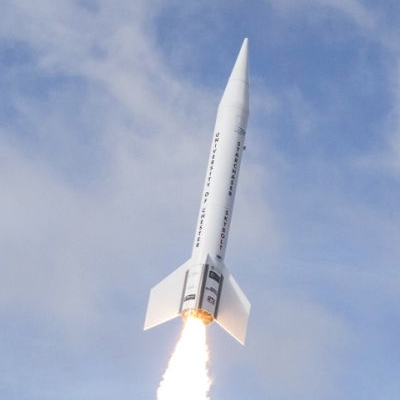
\includegraphics[width=\textwidth]{rocket.png}
  \caption{Rocket}
  \label{fig:sub2}
\end{subfigure}
\begin{subfigure}{.23\textwidth}
  \centering
  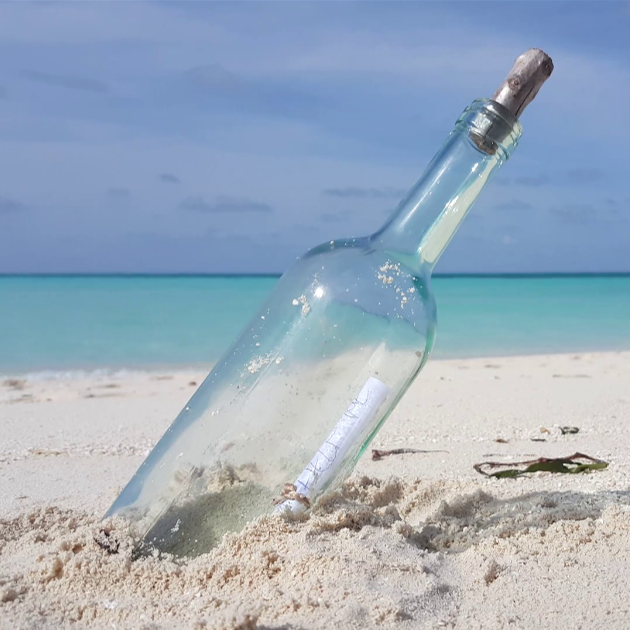
\includegraphics[width=\textwidth]{bottle.png}
  \caption{Bottle}
  \label{fig:sub3}
\end{subfigure}
\label{fig:exampleSimilar}
\caption{Examples of similar classes.}
\end{figure}

\begin{figure}
  \centering
  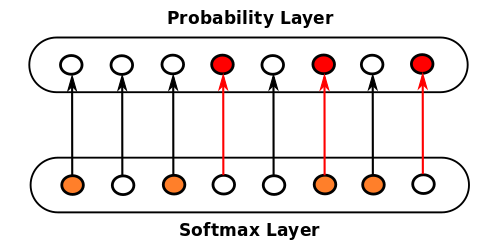
\includegraphics[width=.45\textwidth]{intuition.png}
\caption{Intuition on how probability layer and softmax layer take effect together.}
  \label{fig:intuition}

\end{figure}





% Intuition of probability layer
Probability layer helps by using environment information that original CNNs does not use. When human recognizes an object, both vision and environment information will be used, i.e., what we have seen recently and which objects may appear here. However, CNNs can only make use of visual information while discarding environment information, which makes it extremely difficult to distinguish classes with similar shapes. For example, Figure \ref{fig:sub2} and Figure \ref{fig:sub3} shows images from CIFAR100 for bottle and rocket respectively. It is hard to distinguish these two classes only from images while environment information can easily rule out rocket in most scenarios. 

Figure \ref{fig:intuition} gives intuition on how probability layer utilize environment information. In figure \ref{fig:intuition}, the lower row represents the outputs from softmax layer and the upper row represents the probability layer. The orange nodes stand for the classes with high predicted probability in softmax layer and the red nodes stand for the suggestion from the environment. The prediction from probability layer will be selected from the intersection of the set of red nodes and orange nodes, which rules out confusing classes for CNNs. 
%how to select general model?


\subsection{Perforation}
In this section, we introduce perforation, a pruning method on three levels, i.e. neuron-wise, channel-wise, and layer-wise, as well as class-specific optimization. 

\paragraph{Layer-wise perforation.}
We introduce a global mask to temporally mask out unsalient filters in each iteration based on a pretrained model. Therefore, equation \ref{eq:1} can be rewritten as:
\begin{equation} \label{eq: 2}
    \mathcal{Z}_l = M_l \cdot f(\mathcal{Z}_{l_1} \ast \mathcal{W}_l), \ \ \  s.t. \: l = 1,\: 2, \: \dots, \: L,
\end{equation}
where $M_l \in {0, 1}$ is a mask with a binary value. $M_l = 1$ if the $l$-th layer is salient, and $0$ otherwise. $\cdot$ denotes the point-wise product. By masking out certain layer as zero, we can view it as skip the computation of this layer. This operation will make the input to the next layer to be zero and requires finetuning to continue. Instead, we perforate the skipped layer by previous layers, which can maintain the input tensor size to the next layer and continue prediction without finetuning. Thus equation \ref{eq: 2} can be rewritten as:
\begin{equation}
    \mathcal{Z}_l = g(m_l, f(f(\mathcal{Z}_{l_1} \ast \mathcal{W}_l)), Z_{l-1}), \ \ \  s.t. \: l = 1,\: 2, \: \dots, \: L,
\end{equation}
where
\begin{equation}
    g(x, y, z) = 
    \begin{cases}
        y &\text{se $x = 1$}\\
        z &\text{se $x = 0$}
    \end{cases}
\end{equation}
The problem to prune the most unsalient layers until there are only $K$ layers can be rephrased as an optimization problem:
\begin{equation*}
\begin{aligned}
& {\text{min}}
& & L(Y, h(X; W, m)) \\
& \text{s.t.}
& & ||m||_0 \leq K
\end{aligned}
\end{equation*}
To solve this problem, we provide a heuristic algorithm. In each round, we will remove the layer with smallest negative effect on the final accuracy. Each round can be seperated into many steps and in each step we will remove a single layer while keeping all the other layers. Since perforation is used to recover the feature map size to the layer after the skipped layer, the computation can continue and the final accuracy is still available. Thus in each step, we can get the accuracy after removing the corresponding layer. After iterating through all layers, we can get which layer has smallest negative effect on the final accuracy and remove this layer.

\paragraph{Channel-wise perforation.} Channel-wise perforation could be done in a similar approach with layer-wise perforation. Instead of masking out the whole layer, we adopt a finer granularity with a vector $m_l = \{0,1\}^{C_l}$ as channel-wise mask. The equation \ref{eq:1} can be rewritten as:
\begin{equation} \label{eq: 3}
    \mathcal{Z}_l = f(\mathcal{Z}_{l_1} \ast (m_l \odot \mathcal{W}_l) ), \ \ \  s.t. \: l = 1,\: 2, \: \dots, \: L,
\end{equation}
where $m_l = 1$ if the $l$-th filter is salient, and $0$ otherwise. $\odot$ denotes the channel-wise product. By masking out certain channels as zero, we can view it as skipping the computation of this layer. For the reason of continue computation, we perforate the skipped channels by previous channels. Similar to the heuristic algorithm in layer-wise perforation, we can prune channels in a one-by-one approach.

\paragraph{Neuron-wise perforation.} We choose to increase strides to skip neurons instead of using a mask to identify important neurons in each feature maps. The reason is that, as indicated in xxxxx, this process may introduce irregularity in the computation of neurons and overhead on computation will be introduced. By increasing strides, we can still skip some neurons while there are mature implementation of increasing strides.



\begin{figure*}
\centering
\begin{subfigure}{.2\textwidth}
  \centering
  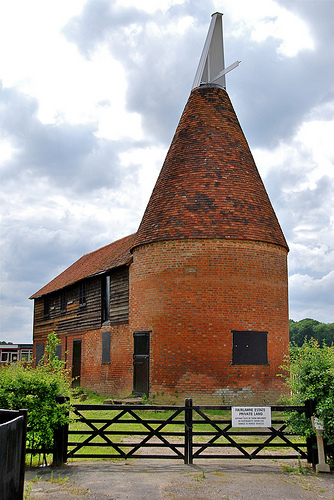
\includegraphics[scale=0.1]{classTypeExample1.jpg}
  \caption{House}
\end{subfigure}%
\begin{subfigure}{.2\textwidth}
  \centering
  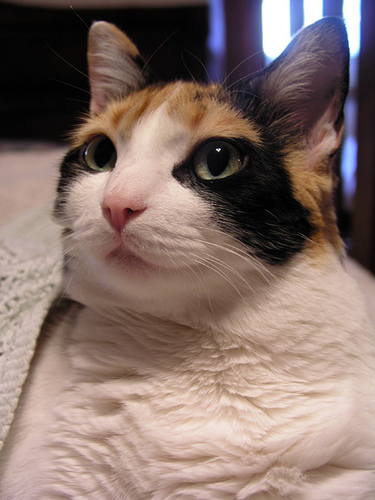
\includegraphics[scale=0.14]{classTypeExample2.jpg}
  \caption{Cat}
\end{subfigure}%
\begin{subfigure}{.2\textwidth}
  \centering
  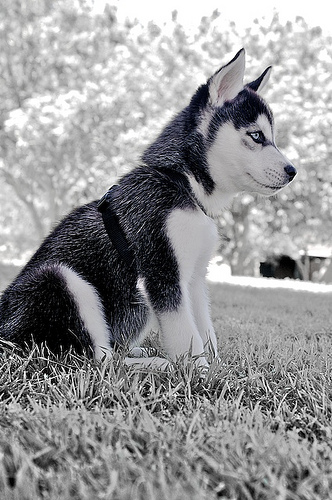
\includegraphics[scale=0.1]{classTypeExample3.jpg}
  \caption{Dog}
\end{subfigure}%
\begin{subfigure}{.2\textwidth}
  \centering
  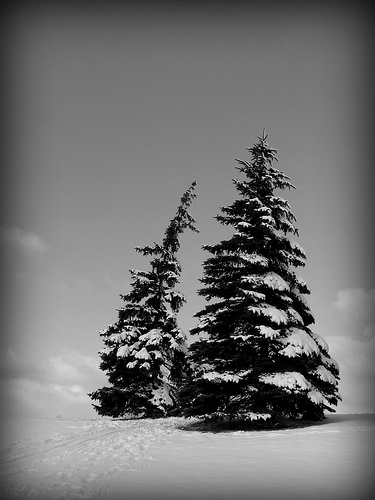
\includegraphics[scale=0.1]{classTypeExample4.jpg}
  \caption{Tree}
\end{subfigure}


\begin{subfigure}{.2\textwidth}
  \centering
  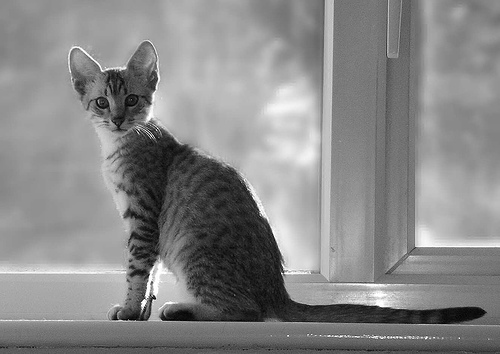
\includegraphics[scale=0.1]{classTypeExample5.jpg}
  \caption{Egyptian Cat}
\end{subfigure}
\begin{subfigure}{.2\textwidth}
  \centering
  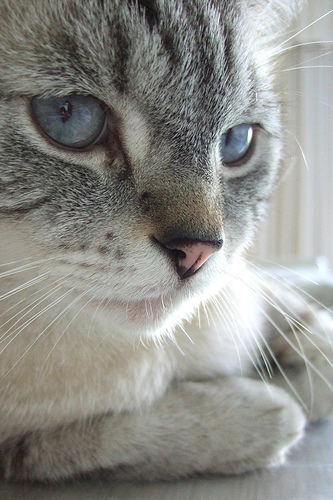
\includegraphics[scale=0.11]{classTypeExample6.jpg}
  \caption{Kitty Cat}
\end{subfigure}
\begin{subfigure}{.2\textwidth}
  \centering
  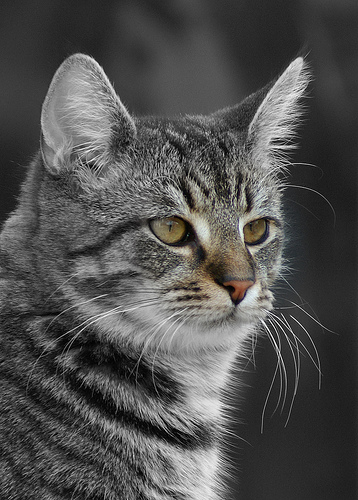
\includegraphics[scale=0.15]{classTypeExample7.jpg}
  \caption{Tiger Cat}
\end{subfigure}
\begin{subfigure}{.2\textwidth}
  \centering
  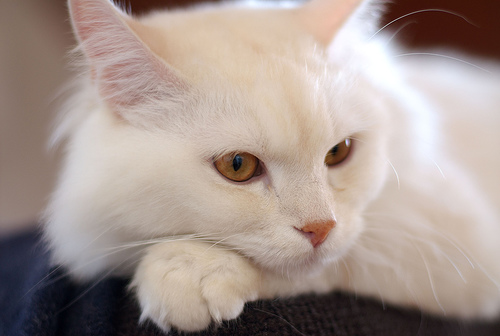
\includegraphics[scale=0.1]{classTypeExample8.jpg}
  \caption{Angora Cat}eq:1
\end{subfigure}

\caption{Set of images showing the class effect. Upper images is easier to distinguish than the lower ones.}
\label{fig:classEffect}
\end{figure*}

\paragraph{Class-specific pruning.} 
We observe that some groups of classes are much harder to classify than others, as indicated in figure \ref{fig:classEffect}. For example, it is much easier to classify house, cat, dog, and tree than distinguishing four different cat species. In fact, distinguishing four different cat species requires expertise in cat species and carefully check on subtle features, i.e. ear size, tail length, coat patterns, and sometimes even personality \cite{cat2018}. Through a series of experiments, we found that classes with low similarity have much higher testing accuracy than classes with high similarity even if the model architecture and the number of classes remain unchanged. Specifically, using a CNN model with 4 convolutional layers and 3 fully connected layers, the accuracy is only 31.49\% to classify baby, boy, girl, man, woman from CIFAR100 while the accuracy would increase to 66.5\% when classifying bottles, bowls, cans, cups and plates. Following along this line of thought, with the same targetting accuracy, models could consume less resource to classify a group of class with high difference. 

To do so, during the pruning process, instead of the original dataset with all possible classes, a specialized dataset with only targetted classes are used and the accuracy on the specialized dataset is used as standard to select the model with least resource consumption and best performance. Evaluations show that the model can achieve the same accuracy with further 20\% less resource consumption to classify house, cat, dog, and tree than distinguishing four different cat species, see section 5. (VALUES TO BE CHANGED)

Also note that class similarity is orthogonal to number of classes since number of classes consider how many classes have appeared in a scenario and class similarity considers how similar the group of classes are to each other, which is orthogonal to number of classes. Thus the class specific pruning could be used simultaneously with probability layer.

\paragraph{Speed up perforation}
In the procedure of pruning, we generate a cascade of models with decreasing accuracy. When redundancy in architecture is abundant, a single step in the perforation may only decrease the accuracy by less than $0.1$\%. However, we may not require a too fine-grained cascade since it indicates a larger number of models and more disk consumption. Instead, SECS service would require the user to define a threshold on the required granularity and adjust the perforation rate during the pruning procedure to maintain a cascade with required granularity. 

We utilize control theory to speed up perforation. When the accuracy remains similar, we will increase the perforation speed, i.e. decrease more channels, layers or increase more strides during the same perforation step.

\paragraph{Search suitable architectures.}
During the procedure of perforation, we can generate a cascade of models with decreasing resource computation and performance. To find the model with targetted accuracy, we do not need to finetune all models. Instead, based on the property of decreasing accuracy, we can test the models in a binary search approach, which would only take logarithm times.

\paragraph{Discussion on reducing resolution}
Reducing resolution has been reported as an effective approach in optimizing architecture \cite{krizhevsky2009learning, fu2017look, howard2017mobilenets}. Reducing resolution indicates the proportional reduction in feature map sizes in all layers and thus both reduce computation and memory consumption proportionally. However, reducing resolution force the reduction in feature maps sizes in a uniformly way across all layers. We argue that reducing uniformly is infeasible since different positions in the architecture has different degree of redundancy. Instead, perforation could reduce feature map sizes, channel numbers, and layer numbers according to the redundancy in different positions and prune the architecture correspondingly, which would introduce more optimization with less penalty in accuracy. Actually, reducing resolution is equivalent to add a pooling layer before the whole architecture or increase strides in the first layer, which is covered by perforation and could be selected when feasible.

Also note that in MobileNet \cite{howard2017mobilenets}, reducing resolution is utilized by adding an extra hyper-parameter selected by hand, which becomes an obstacle for users who are not familiar with CNN architectures. Instead, perforation selects in an end-to-end automatic way and hide procedures from user.



\subsection{Profiler}
Use online learning method to record and update the distribution consistently. Every C minutes, we will check whether the distribution has changed using xxx statistic formular.

\subsection{Sharing}
It has been identified by existing works that multiple applications could process same input stream concurrently. Thus the same classification results could be shared among all applications instead of repeating the computation by each applications. To do so, we build an interface \textit{AppListenser} to get request from all applications and feed back same results to everyone, see section 4.2.


\subsection{Scheduling Model}
The task of scheduling model is to select a series of models to process the image stream under a resource constrain. The target is to maximize the accuracy while trying to use less energy for each image. The choice is between a cascades of models with different accuracy and different energy consumption. To solve this optimization problem, we build a heuristic algorithm, in Algorithm 1 to allocate energy for each input image, choose the most suitable model given the per frame energy, and wrap all the decisions automatically.

With a process rate of $F$ frames per second and current available energy budget, the perframe energy can be estimated. In concrete, $AllocateEnergy$ (line 11) will retrieve the expected running time and estimate per frame energy by averaging the available energy over all remaining time. Given per frame energy budget and recorded class skew, $ChooseModel$ will return the best model. If no class skew exists, $ChooseModel$ do not need to consider retraining and will choose the model with highest accuracy given current energy budget. When there is class skew, the $ExistedRetrainedModel$ will check whether there are retrained model for current class skew and return a suitable model. When there is no retrained model on disk, the architecture will choose between retraining last few layers and using probability layer. Since retraining is costly, we expect to have enough energy to run that retrained model for at least 10 minutes, otherwise it is more feasible to avoid retraining and use probability layer directly.

The scheduler will wrap up all the algorithms in scheduling model and give the most suitable model. For every input image $i$, The scheduler needs to get the class skew report $r$ from profiler. In the high accuracy mode, enough energy is given to each image such that more freedom in choice of models is allowed. In the efficiency mode, $allocateEnergy$ will estimate per frame energy according to expected remaining running time. Given this per frame energy and class skew report, the chooseModel will give the best model $m$ and the corresponding accuracy $a$. Finnaly, the $scheduler$ will call $execute(i,m)$ to run the model $m$ on input image $i$.


\begin{algorithm}
 \caption{Scheduling Model}
  \begin{algorithmic}[1]
    \Function{Scheduler}{$i, r, mode$}
        \State $AE = RemainEnergy()$    
        \If {mode == HIGHACCURACY}
            \State $PFE = AE / 600 $ 
        \ElsIf {mode == EFFICIENCY}
                \State $PFE = allocateEnergy(AE)$
        \EndIf
            \State $a, m = chooseModel(PFE, r)$  
            \State $execute(i,m)$        
    \EndFunction

    \Function{allocateEnergy}{$AE$}
        \State $n = RemainingTime()$
        \State $PFE = AE/n$
        \State \Return $PFE$
    \EndFunction
        \Function{chooseModel}{$PFE, r$}
        \If{$Parse(r) == NoSkew$}
            \State $a, m = getModel(PFE)$ 
        \ElsIf{$Parse(r) == Skew$}
            \State $a,m = ExistedRetrainedModel(r, PFE)$
            \If{$m == NULL$}
                \If{$PFE > \Delta E/600 + FrameCost(m,r)$}
                    \State $a,m = retrain(m,r)$
                \Else
                    \State $a,m = probabilityLayer(m,r)$
                \EndIf
            \EndIf
        \EndIf
        \State \Return $a,m$
    \EndFunction

    
\end{algorithmic}
\end{algorithm}




\section{Implementation}
\subsection{Architecture}

\begin{figure} 
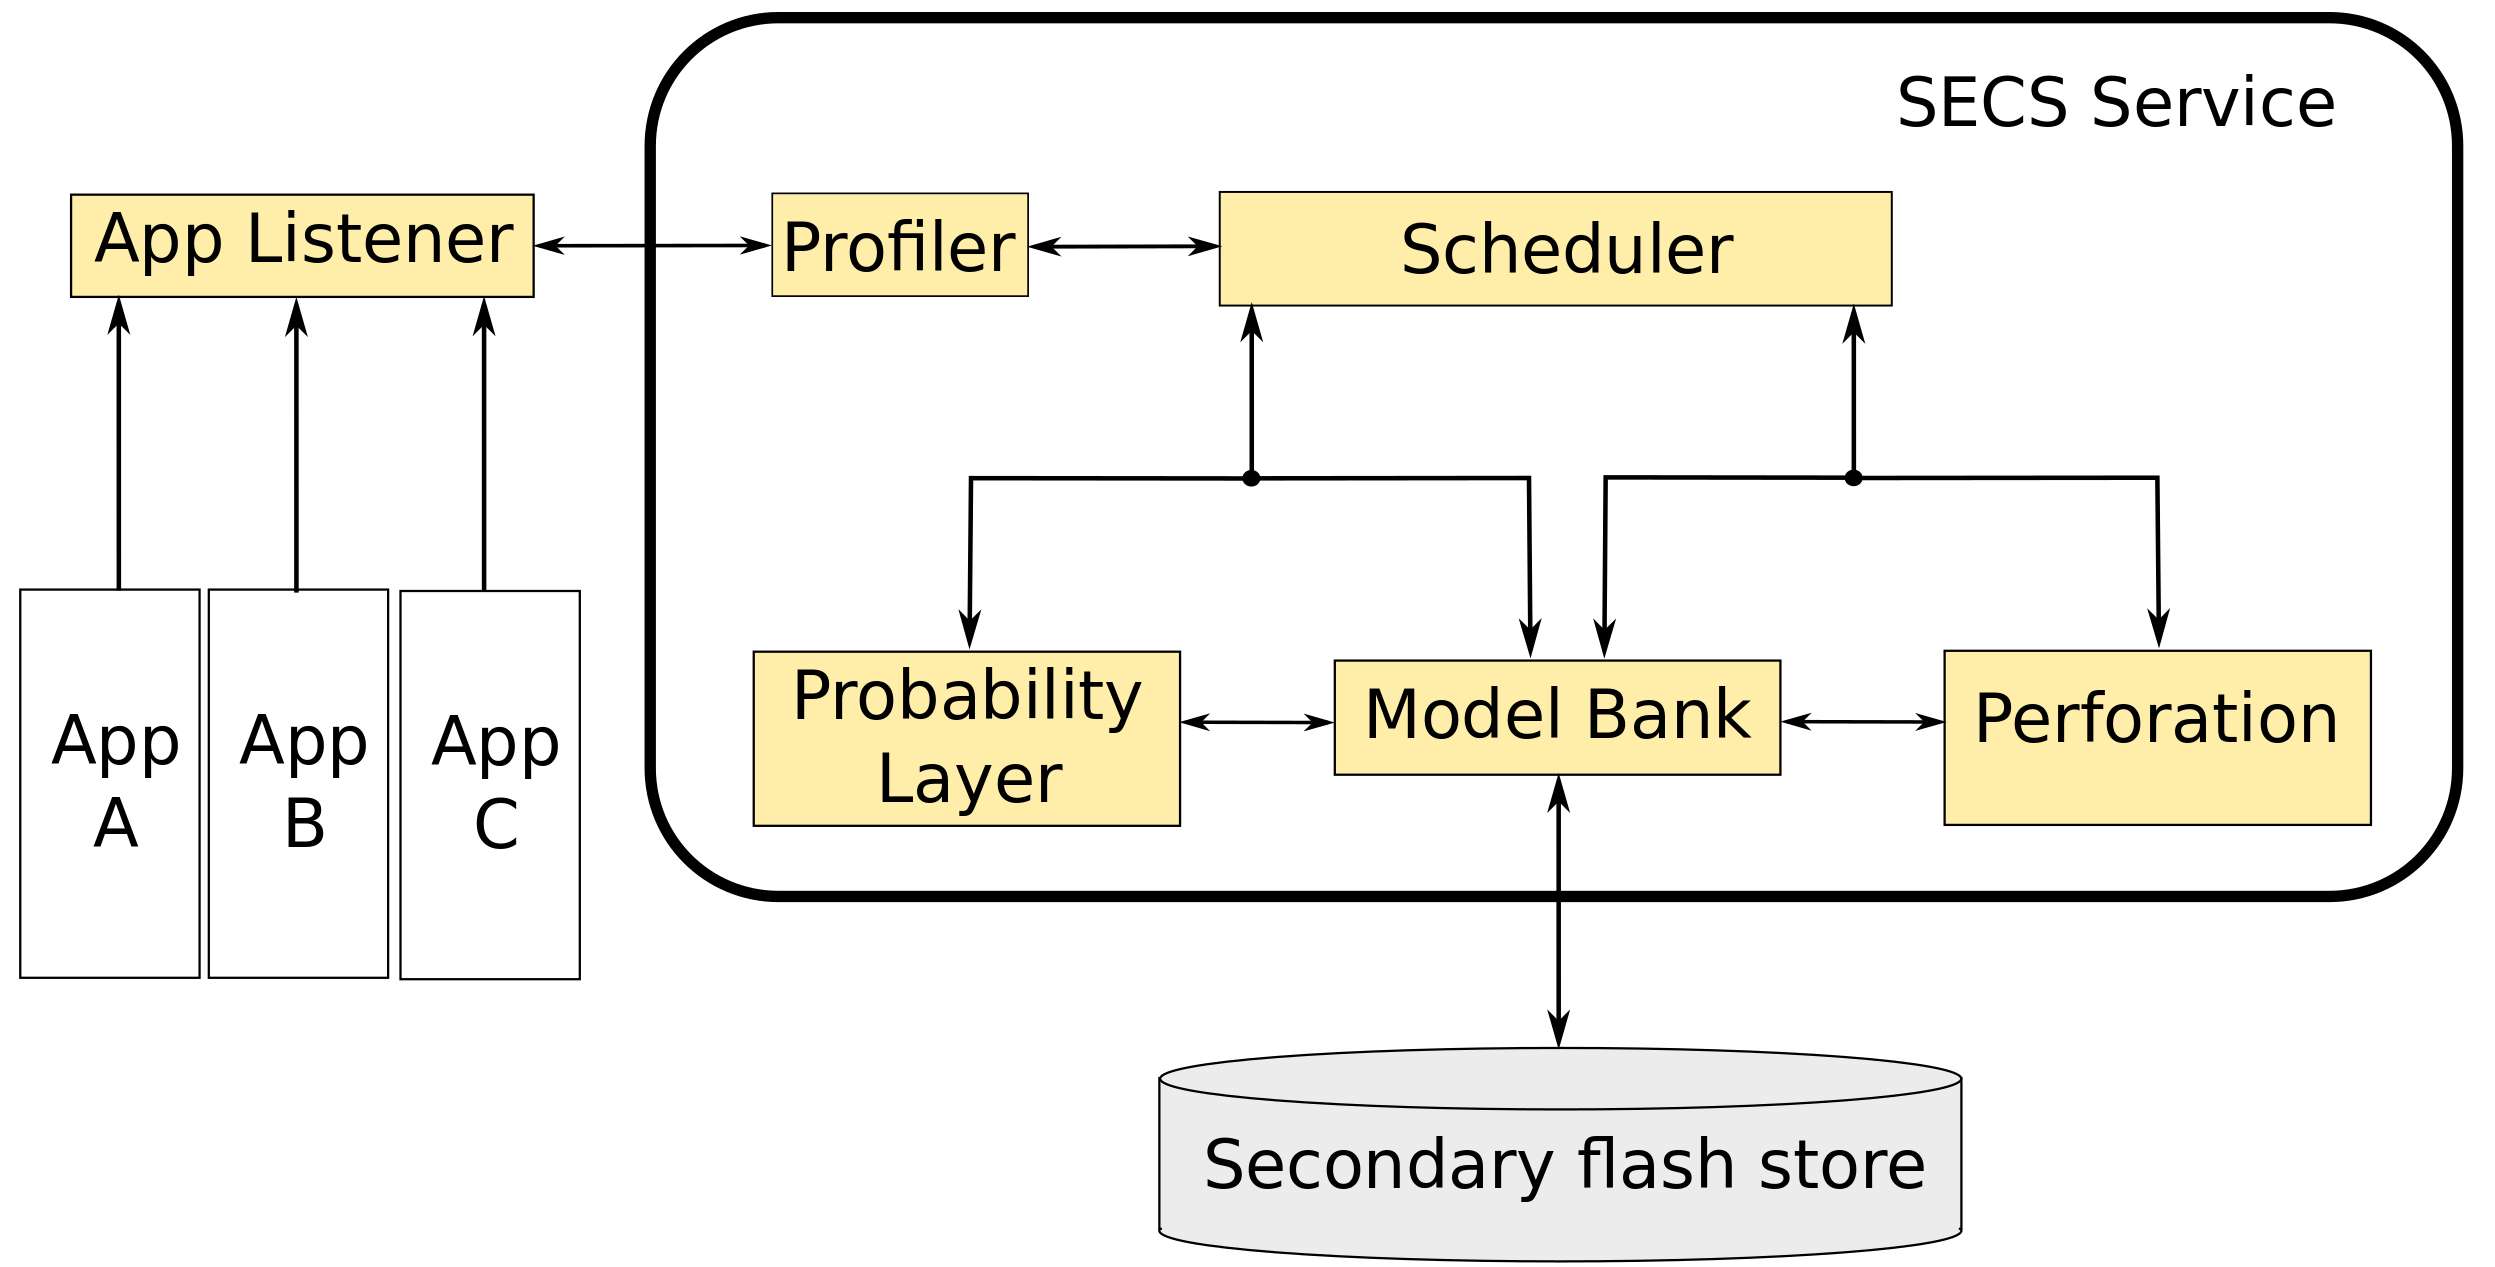
\includegraphics[scale=0.095]{architecture.png}
\caption{System architecture.}
\label{fig:Architecture}
\end{figure}

We implement SECS as a end-to-end classification service with Tensorflow \cite{tensorflow2015-whitepaper}. Figure \ref{fig:Architecture} shows the architecture of the system. 

The image classification service consists of the following modules. The \texttt{AppListener} maintains a threadpool, summarizes the requests from upper-level applications into a stream, and forwards the stream into \texttt{profiler} for further procedure. During runtime, the \texttt{profiler} maintains current class distribution and effectively detect class skew. Once class skew is detected, the \texttt{profiler} will either call existing adapted model from \texttt{model bank}, or require the \texttt{probability layer} to efficiently adapt the model. The classification results will be feed back to \texttt{profiler} which will both respond the \texttt{AppListener} and update runtime class skew. During cold time, the \texttt{profiler} will check whether a class skew has appeared more frequently than a pre-defined threshold, and call \texttt{perforation} to generate class-specific pruned models for more optimized classification in the future.


\subsection{Image classification service}
\paragraph{Probability layer.}
We build probability layer by adding a single extra layer after the original model. The probability layer could be implemented as a variable using \textit{tf.get\_variable} with dimension \textit{1xn}. The probability layer will be initialized with the runtime class skew recorded by \texttt{profiler}, which is freely available and no overhead is introduced. The sum of this variable and the original softmax layer will replace the original softmax layer and used as the classification results. 

\paragraph{Perforation.}
There are three levels of perforation, i.e. neuron-wise, channel-wise, and layer-wise. Generally, we speedup computation by skipping several carefully selected positions. The reduced feature map sizes or number of channels will obstacle the forward computation in CNNs. Perforation is used to make up the holes that has been skipped using values from adjacent positions. 

Specifically, we implement neuron-wise perforation by increasing strides to reduce computation and use interpolation methods to recover the feature map sizes. By default, \textit{tf.image.resize\_images} and nearest neighbor algorithm is used for interpolation. 

To implement channel-wise perforation, we maintain a global 0-1 mask for all channels indicating whether or not keep the specific channels according to their importance towards accuracy. After masking out the channels, we fill the hole with adjacent channels. \textit{tf.split} can split tensors channel-wise effectively. These splited tensors can be concatenated using \textit{tf.concat} to recover the original number of channels and enable the forward computation with original weights. Layer-wise perforation could be implemented in a similar approach.


\paragraph{Profiler}
Use online learning method to record and update the distribution consistently. Every C minutes, we will check whether the distribution has changed using xxx statistic formular.


\begin{table}
    \centering
    \begin{tabular}{l|c|c|c|c}
        \hline
        Model & Class skew  & Comp. & Mem. & Acc. \\
        \hline
        fake & N/A & 2.3 & 123 & 76.5 \\
        ? & ? & ? & ? & ? \\
        ? & ? & ? & ? & ? \\
        ? & ? & ? & ? & ? \\
        \dots & \dots & \dots & \dots & \dots \\
        \hline
    \end{tabular}
    \vspace{1em}
    \caption{Model bank.}
    \label{tab:modelBank}
\end{table}

\paragraph{Model bank.}
All the generated models are stored in model bank, as table \ref{tab:modelBank}. Each entry contains the status of a single model, including whether it is a general model or class-specific pruned model, required computation and memory, and the accuracy. \textit{N/A} represents no class skew used in the model. The model bank will support the runtime decision from \texttt{profiler} and only models at the Pareto-optimal bound will be selected for service.




\paragraph{AppListener.}
As the interface, \texttt{AppListener} receives messages from applications containing the input image and required accuracy. Since all real-time applications on the same mobile platform essentially analyze the same input stream, opportunities are created to share the same classification results. To synchronize the requests from all applications, the input images received within a time period will be synchronize into a single one and all related requests will get the same results. As indicated by \cite{jiang2018mainstream}, the choice of this threshold represents a tradeoff between resource efficiency and accuracy. By default, we choose the threshold as a half second.

\subsection{APIs and patches to the application code}
To simplify the usage of SECS service, the user only need to use the interface \textit{request()}, providing the input image and required accuracy. Both classification and pruning will be done by SECS service automatically.








\section{Evaluation}








\subsection{Probability Layer}
A series of experiments on various kind of specialized datasets have shown the effectiveness of probability layer. CIFAR100 is a prevalent benchmark for various kind of CNN models, which has 100 classes, a training dataset with 500 images per class, and a testing dataset with 100 images per class. To mimic the runtime distribution, we generate a specialized dataset manually. For example, in generation of a specialized dataset with 80\% data skew and 10 domain classes, we would use 1000 images from the testing dataset according to these 10 domain classes, and randomly select 250 images from other classes. We trained the model on original CIFAR100 training dataset and test the model on various kind of specialized datasets with different number of domain classes and selection of domain classes. We also take into account that the selection of domain classes because the choice of labels have strong effect on the test accuracy, even if we keep the number of domain classes unchanged. Actually some classes are easier to classify than others. To eliminate this random effect, we will choose different groups of labels for each number of domain classes.

Figure 
%\ref{fig:ProbabilityLayer} 
summarizes the results. As a benchmark, the test accuracy on the CIFAR100 testing dataset without probability layer is 73.74\%. If the number of domain classes is 2 and we choose the label 0 and 1, the accuracy without probability layer is 88.12\%. The difference between specialized testing accuracy 88.12\% and the overall accuracy 73.74\% is due to selection of classes. If we change the label pair from (0,1) to (3,5), the accuracy would also change from 88.12\% to 61.39\%. However, in both case, the accuracy with probability layer are 98.51\% and 99.01\%, which performs very well consistently. 

Then we increase the number of domain classes from 2 to 5 and choose domain classes as 0 to 4 and 5 to 9 respectively. This time, the effectiveness of selection of domain classes appears again. If we set domain classes as 0 to 4, the accuracy without probability layer would be 66.33\%. If we set domain classes as 5 to 9, the accuracy would be 81.06\%. The accuracy with probability layer in these two cases would be 93.03\% and 97.01\% respectively. The benefit of probability layer are 26.70\% and 15.95\% respectively.

When we increase the number of domain classes further to 10, the effectiveness of probability layer would still be dramatic. We choose 0 to 9, 10 to 19, 20 to 29 as domain classes. The accuracy without probability layer would be 75.35\%, 67.16\%, and 75.84\%. The accuracy with probability layer would be 94.21\%, 91.41\%, and 92.22\%. The benefits are 18.86\%, 24.26\%, and 16.38\%.

To explore the interaction between probability layer and number of domain classes, we increase the number of domain classes gradually from 2 to 100. The benefit disappears gracefully. When number of domain classes is less than 20, the benefit are above 18\%. Even if we have 40 domain classes, the benefit is still around 10\%. When there are 60 classes, there are 5\% benefit. Since we do not need retrain, these benefit are almost free. We do not need extra memory or energy and we have not introduced any extra latency. The only thing that we need is the run time distribution, which could be collected easily through an in-memory record.




Experiments show the significant of \textit{probability layer} over \textit{naive mask}. Figure \ref{fig:NaiveMask} shows the comparison between probability layer and naive mask under different configurations. The red dash line represents the original accuracy without probability layer and naive mask, which is 74.57\%. When the number of domain classes is 10 and the distribution skew is 50\%, the accuracy with probability layer is 75.28\%, while the accuracy with naive mask is only 47.49\%. Thus probability layer has a positive effect even if the distribution skew is only 50\%, while the naive mask has a strong negative effect in this context. As we increase distribution skew gradually, the accuracy with probability layer and naive mask keeps increasing. Only after the distribution skew becomes larger than 77.67\%, naive mask starts to show positive effect on accuracy while probability layer keeps showing positive effect in all settings. As distribution skew approaches 100\%, the effect of naive mask catches probability layer up, since the true labels start to only exist in domain classes. In short, probability layer is a generalization of naive mask and shows benefit over original model and naive mask consistently.

\begin{figure}
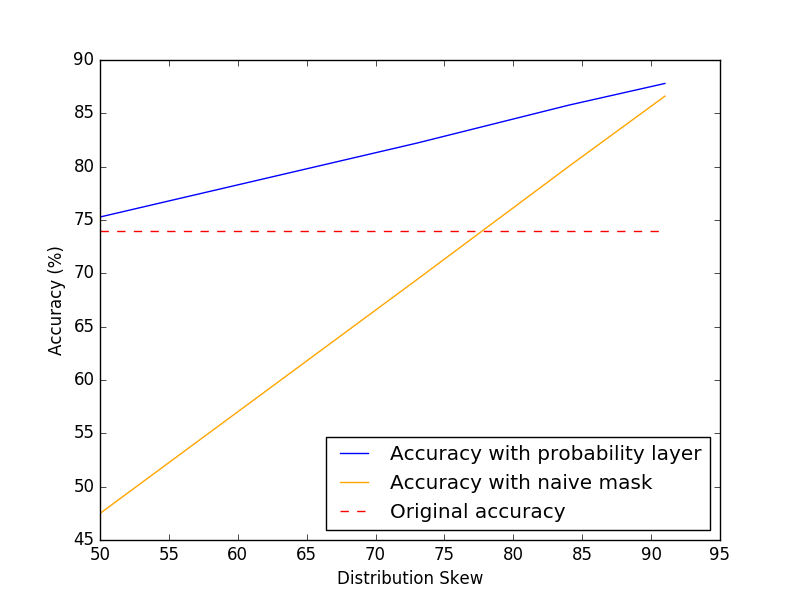
\includegraphics[scale=0.43]{figure_1-1.png}
\caption{Comparison Between Probability Layer and Naive Mask}
\label{fig:NaiveMask}
\end{figure}


\begin{figure}
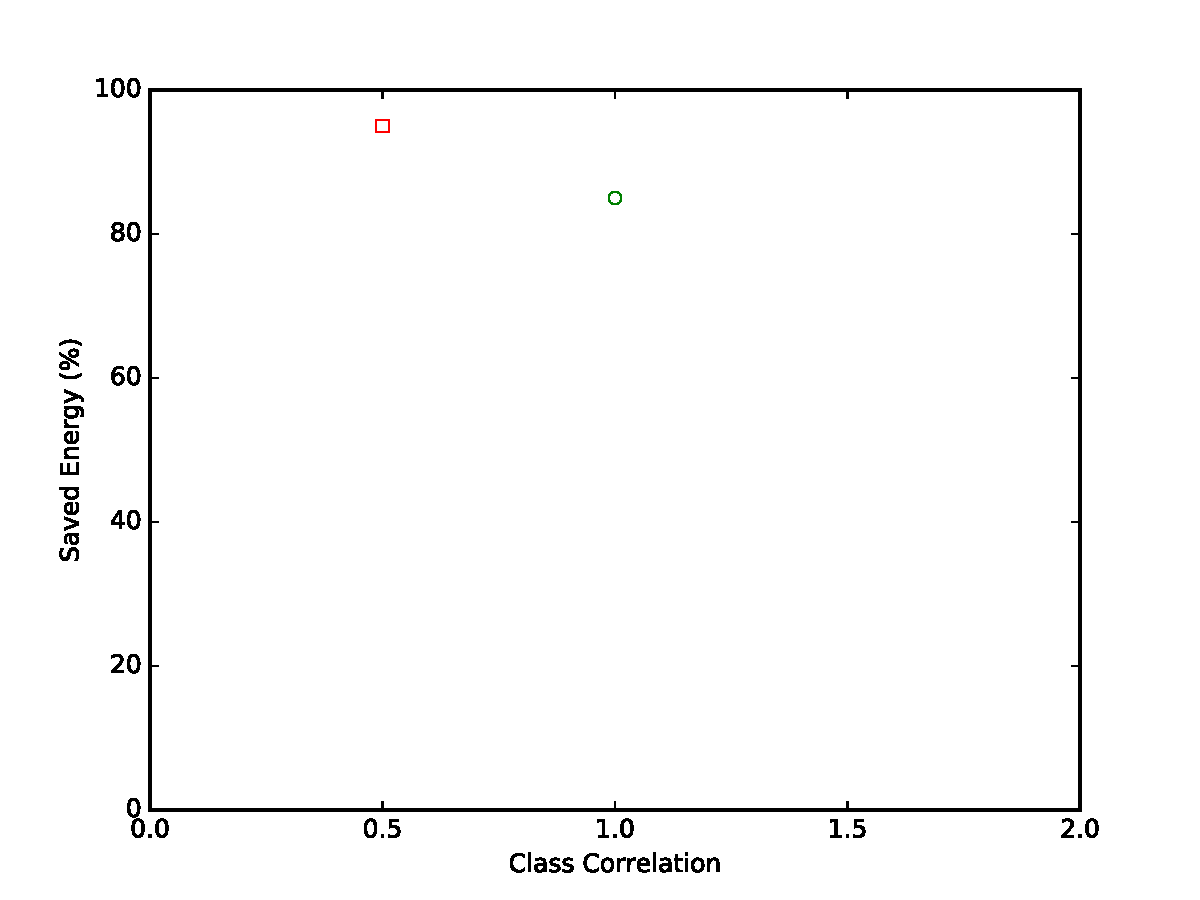
\includegraphics[scale=0.43]{savedEnergy.ps}
\caption{Saved Energy}
\label{fig:savedEnergy}
\end{figure}


\subsection{Energy efficiency}
Considering class correlation can save more energy than only considering number of classes. Fig \ref{fig:savedEnergy} shows the energy saved by class correlation. We generate a subset from CIFAR100 with 2 classes and different class correlation. The accuracy of VGG16 on CIFAR100 is 70.48\%. We simplify VGG16 and reduce layers until the testing accuracy on specialized dataset is lower than 70\%. Considering the innegligible impact of class correlation on testing accuracy, the experiments are done by different class correlation and, for each class correlation, the classes are selected randomly and the experiments are repeated for twenty times to get an average accuracy. When the class number is two and class correlation is $1$, we need a model with one convolutional layer and two fully connected layer to get the accuracy as $72.9\%$. Thus we only need to consume $85\%$ computation to get the same accuracy as the VGG16 with $19$ layers. If we decrease the class correlation to $0.5$, we only need a single fully connected layer to achieve 74.6\% accuracy. In this case, only $5\%$ computation of VGG16 is consumed. Thus, as we decrease class correlation from $1$ to $0.5$, the energy consumption is decreased by $66\%$



We implemented probability layer on DenseNet \cite{huang2017densely} and evaluated the CNN model with probability layer, i.e., \textit{PCNN}, on specialized datasets with various number of classes and class distribution. We choose DenseNet as the base model since it is the state-of-the-art and has similar results with other state-of-the-art models, i.e., GoogLeNet \cite{szegedy2015going} and ResNet \cite{he2016deep}. We reimplemented the DenseNet on Tensorflow \cite{abadi2016tensorflow} and trained the model on CIFAR100 \cite{krizhevsky2009learning} from scratch. The \textit{specialized dataset} is generated from CIFAR100 \cite{krizhevsky2009learning}, which originally has $100$ classes with equal weight. 

\textbf{Transfer Learning.} Following the published practice \cite{doersch2015unsupervised, han2016mcdnn, oquab2014learning, shen2016fast, yosinski2014transferable}, all fully-connected layers after convolutional layers are finetuned on the generated dataset with same class distribution as the testing dataset. To eliminate the effect of the epoch, we used three different epochs, i.e., $1$, $5$, and $30$. The maximum epoch is $30$ because latency and energy efficiency are considered.

To show the potential of PCNN, we evaluate probability layer on specialized datasets composed of a various number of classes and class distributions. We begin our experiments by showing that different class combinations have significant influence over the accuracy and probability layer can bring in benefit and perform better than transfer learning on all class combinations. Then we show that probability layer can improve accuracy for any number of classes and make use of unbalanced distribution. We proceed to show that most of the images will have predicted probability higher than $75\%$, which are called \textit{high-confidence images}, and the accuracy among these high-confidence images is $84\%$. Finally, we demonstrate that probability layer is complementary to acceleration methods through combining probability layer with spatial redundancy elimination approach \cite{figurnov2016perforatedcnns} to achieve decreased computation and improved accuracy.

\subsection{Class effect}
We explore the effect of class combinations and compare the performance of probability layer and transfer learning on various class combinations. Fixing the number of classes as two, we randomly selected five class combinations and compare the original model, model after transfer learning, and the model with probability layer, see figure \ref{fig:classEffectExamples}. We see that with the same model, different class combinations may have dramatically different accuracy. While the original model can achieve a accuracy as 83\% for classifying chair and cup, the accuracy for beaver and bear is only 52.5\%. We can also observe that both transfer learning and probability layer can bring in benefit no matter which two classes compose the dataset while probability layer generally performs better than transfer learning. In the randomly selected five class combinations, probability layer can provide an additional benefit of $2.16\%$ on average. Note that for fox and pine, transfer learning provides a slightly better accuracy than probability layer. We believe that this is due to randomness, especially when considering that transfer learning performs better on all other class combinations. 

Figure \ref{fig:classEffectSummary} gives a summary of the performance of all three models on the specialized dataset with two and five classes. The figure shows the result from $100$ randomly selected class combinations. We see that, on the original model, while the average accuracy for classifying two classes is $70\%$, the minimum accuracy could be $45\%$ and the maximum accuracy can reach $83\%$, which shows that the accuracy of classifying two classes could change dramatically even using the same model. This observation also holds for transfer learning and probability layer. We can also note that the average accuracy of probability layer is much higher than transfer learning. 

\begin{figure}[t]
    \begin{subfigure}[b]{0.47\textwidth}
        %\centering
        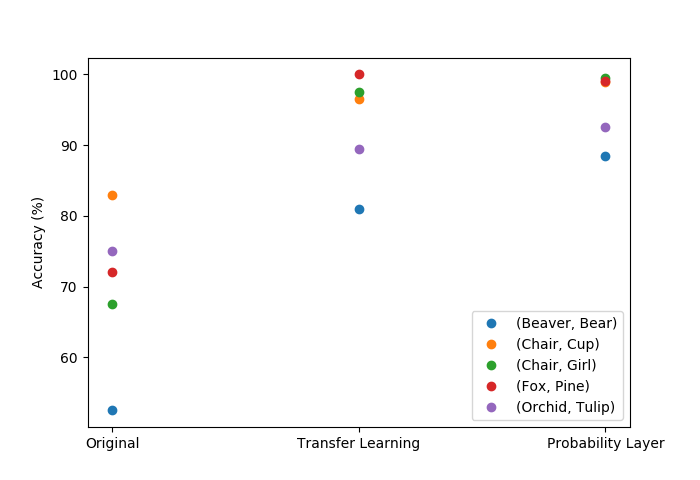
\includegraphics[width=\textwidth]{classEffectLine.png}
        \caption{Concrete examples}
        \label{fig:classEffectExamples}
    \end{subfigure}
    \begin{subfigure}[b]{0.47\textwidth}
        %\centering
        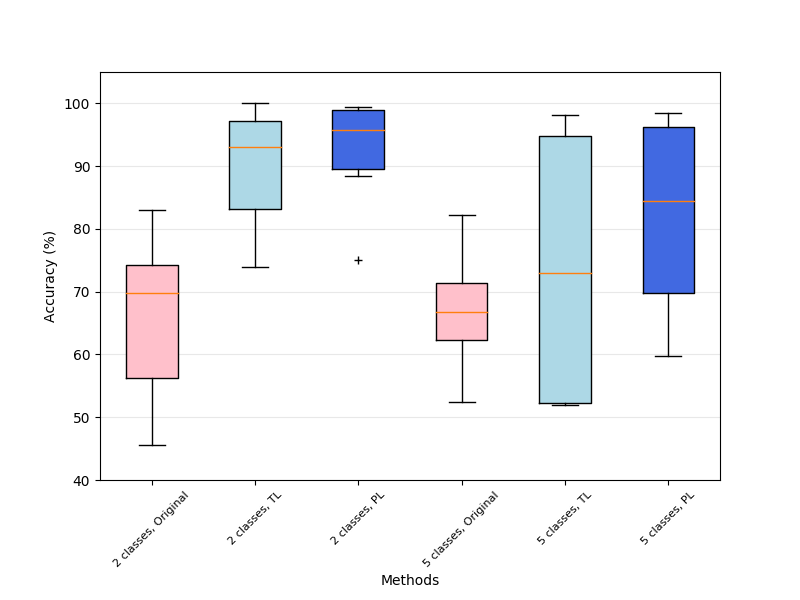
\includegraphics[width=\textwidth]{classEffect.png}
        \caption{Summary of class effect}
        \label{fig:classEffectSummary}
    \end{subfigure}
    \caption{Class effect on the original model, the model after finetuning, and the model with probability layer.} \label{fig:classEffect1}
\end{figure}
\subsection{Results on specialized datasets with only majority classes}

% Third paragraph: Experiment setting
We explore probability layer's ability on making use of environment when there are only a few majority classes. For each number of classes, we randomly sampled $100$ subsets of classes and present the average accuracy in figure \ref{fig:PLvsRetrain}. We see that significant benefit has been achieved by probability layer for all number of classes. When there are 5 classes, an increase of more than $20\%$ can be achieved without any finetuning. Another point worth noting is that the benefit diminishes gradually as the number of classes increases. Even if there are $40$ classes, a benefit over $10\%$ could still be observed. This shows a significant advantage over previously published results \cite{shen2016fast}, in which no benefit exists when there are more than $15$ classes.
 
We compare our results with transfer learning in figure \ref{fig:PLvsRetrain}. For every specialized dataset, we finetune the model for $5$ rounds on a training dataset with the same class combinations and class distribution as the testing dataset. For all selected class numbers, probability layer performs better than transfer learning. This advantage of probability layer over transfer learning increases as the number of classes increase. We contribute this phenomenon to the fact that PCNN has seen more images than transfer learning. Existing papers \cite{yosinski2014transferable} has also reported that transfer learning may destroy the co-adaption between layers and deteriorate the performance on prediction. Another point worth noting is that when the number of classes increases over $90$, retraining would bring worse accuracy than the original model without retraining. In contrast, the probability layer can still bring 2\% advantage over the original model. We believe the reason is that the deterioration of co-adaption between layers leads to a decrease in accuracy and the reduction in the number of classes cannot make up this deterioration when the number of classes is $90$, which is almost same as the original class numbers. Probability layer does not need finetuning and thus avoid this problem. All these observations indicate that probability layer has better ability in using various environment.


\subsection{High confidence, high accuracy}
We justify our design of threshold in probability layer by exhibiting the percentage of images with predicted probability layer higher than the various threshold and the accuracy of these images, see figure \ref{fig:threshold}. While the original DenseNet has top-1 accuracy as $73\%$, the accuracy increase to $83\%$ when we set the threshold $\omega$ to be $75\%$. When we increase furtherly the threshold $\omega$ to be $99\%$, the accuracy would increase to $95.01\%$. Thus when a model has strong confidence in its prediction, we should better believe in the model instead of rescaling. 

We also note that a large portion of images can get a high predicted probability from the original model. For instance, there are more than 60\% images get predicted probability higher than 95\%. For these images that the original model has strong confidence in its prediction, the probability layer will not interfere with the decision. The probability layer will step in when the original model is not sure and give suggestion to the probability layer according to the environment information. 


\begin{figure}[!tbp]
  \centering
  \begin{minipage}[b]{0.49\textwidth}
        \centering
        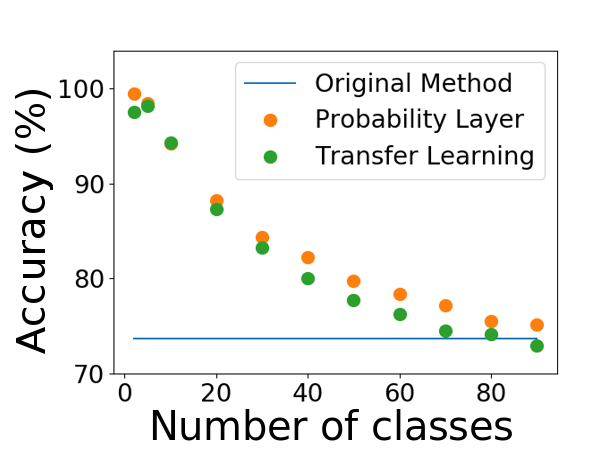
\includegraphics[width=\textwidth]{PLvsRetrain.png}
        \caption{Performance on different number of classes}
        \label{fig:PLvsRetrain}
  \end{minipage}
  \hfill
  \begin{minipage}[b]{0.49\textwidth}
        \centering
        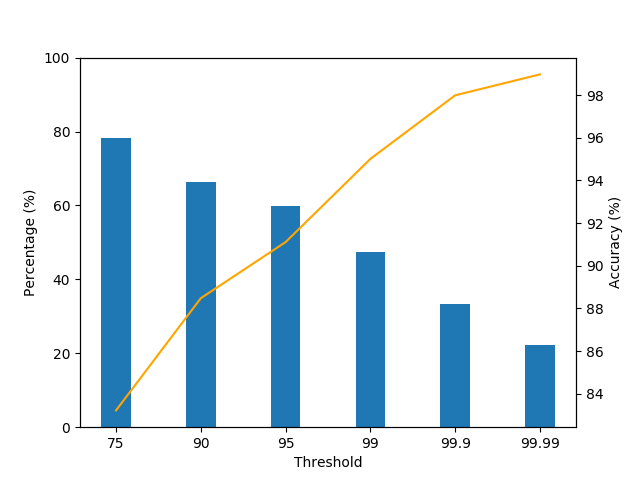
\includegraphics[width=\textwidth]{threshold.png}
        \caption{Threshold}
        \label{fig:threshold}
  \end{minipage}
\end{figure}



\subsection{Results on specialized datasets with both majority and minority classes}
We evaluate the probability layer on the noisy environment, in which a few major classes occupies most of the images while a huge number of minority classes also appear. Figure \ref{fig:variousDistribution5} and figure \ref{fig:variousDistribution10} shows the results when the numbers of majority classes are five and ten respectively. While the weight of majority classes increases from $50$\% to $100$\%, probability layer performs consistently better than the transfer learning for $5$ or $1$ rounds. Even if we finetune the model for $30$ rounds, probability layer still performs better when the weight of major classes is relatively small. When the weights increase further, the advantage of finetuning for $30$ rounds is at most $0.5$\%. Considering the intensive energy-consumption and time latency of retraining for $30$ rounds, this benefit of $0.5$\% advantage is not so significant, especially on devices which require the real-time response and has strict energy budget. We should also note that retraining for $1$ rounds would make the accuracy to be much lower than original model when the weight of major classes is less than 75\%. Since we need to choose a method before we start in automatically using environment information, we can conclude that probability layer is the most suitable method.


\begin{figure}[t]
    \centering
    \begin{subfigure}[b]{0.49\textwidth}
        \centering
        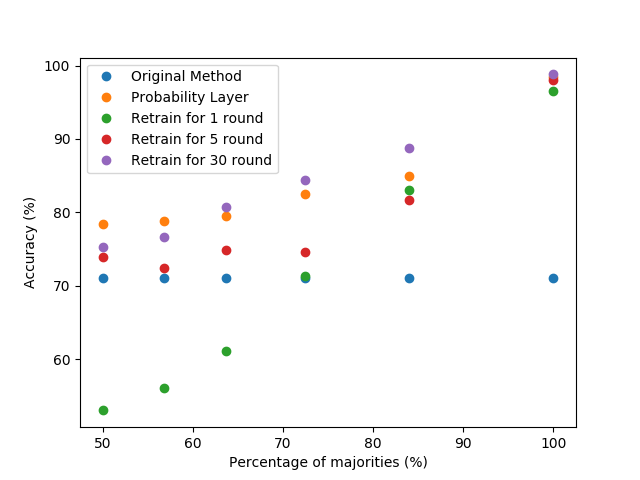
\includegraphics[width=\textwidth]{variousPercentage5.png}
        \caption{Five classes with various distribution}
        \label{fig:variousDistribution5}
    \end{subfigure}
    \begin{subfigure}[b]{0.49\textwidth}
        \centering
        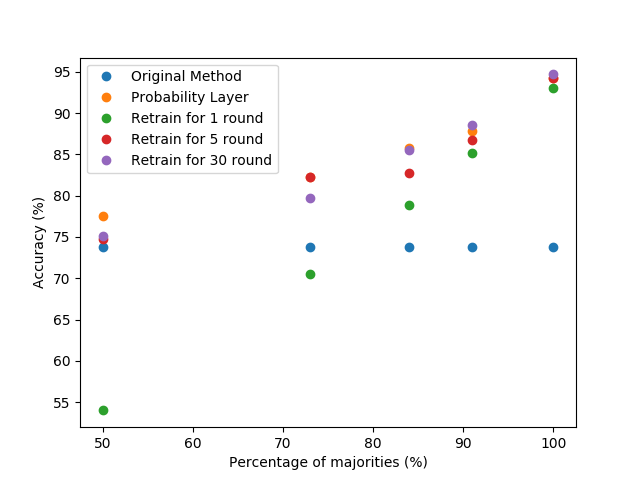
\includegraphics[width=\textwidth]{variousPercentage10.png}
        \caption{Ten classes with various distribution}
        \label{fig:variousDistribution10}
    \end{subfigure}

    \caption{Probability layer on denseNet}\label{fig:complex}
\end{figure}


\subsection{Combining acceleration methods}
A promising way to achieve high speed up and accuracy is to combine acceleration methods with probability layer. For this to succeed, the acceleration methods should utilize different types of redundancy in the network. In this section, we verify that probability layer can be combined with an acceleration method of using spatial redundancy, \textit{PerforatedCNN} \cite{figurnov2016perforatedcnns}, to achieve high speed up while increasing top-1 accuracy.

We reimplemented the PerforatedCNN \cite{figurnov2016perforatedcnns} on DenseNet. PerforatedCNN makes use of spatial redundancy in the image by skipping evaluation in some of the spatial positions. Different from other methods in using spatial redundancy, i.e., increasing strides, PerforatedCNN will interpolate these skipped positions using nearest neighborhood, such that the output size will be unchanged. In this way, the architecture remains same and no finetuning is needed. The shortage of PerforatedCNN is that it may introduce a huge decrease in accuracy. Our experiments show that this drawback of PerforatedCNN could be made up by probability layer. Thus combining probability layer with other acceleration methods can both decrease computation and increase accuracy.

We first apply the probability layer to the network. Then we apply the spatial redundancy elimination methods to this network. In the whole process, no finetuning is needed. The PerforatedCNN is tested at the theoretical speedup level of 2x. The testing dataset contains $5$ randomly selected classes with equal frequency. The results are presented in the table \ref{tab:my_label}. Due to class effect, the original model will give a top-1 accuracy of $67.9\%$, which is slightly lower than the average accuracy of DenseNet on CIFAR100. With the probability layer, the model without finetuning can increase the top-1 accuracy dramatically to be $98.4\%$. The PerforatedCNN will give a top-1 accuracy of $48.19\%$ if we choose the theoretical speedup level of 2x, which is similar to the results reported in PerforatedCNN \cite{figurnov2016perforatedcnns}. Adding the proposed method, the PerforatedCNN can give a top-1 accuracy of $92.20\%$ while decreasing computation by half, which shows that probability layer complements spatial redundancy elimination methods perfectly and provides a promising perspective of combining probability layer with other acceleration methods.

%Considering that the accuracy of previously published acceleration methods always decrease the accuracy, this combined method shows great potential and 



\begin{table}[h]
    \caption{Summary}
    \label{tab:my_label}

    \centering
    \begin{tabular}{ ccc } 
     Method & Mult. $\downarrow$ & Top-1 Accuracy \\ 
     \hline
     Original Model & 1.0x & 67.79\% \\
     Probability Layer & 1.0x & 98.4\% \\ 
     Perforation & 2.0x & 48.19\% \\ 
     \hline
     Combined Method & 2.0x & 92.20\%
    \end{tabular}
\end{table}


\subsection{Detection overhead}
The fundamental of using runtime distribution is detecting runtime distribution, mainly focused on the number of classes and what classes are appearing. Profiler is the component in \textit{SECS} taking care of this detection. As images come, full models will classify these images and profiler will store the results. For every $120$ processed images, the profiler will calculate the distribution of these classified images and compare with the distribution for last $120$ images. We choose $120$ because generally we will process $1$ image per seconds and $120$ images will represent the distribution of classes in two minutes. Assuming there are $n$ classes in the full model, the frequency of each class will be recorded as $f_i$, which is the proportion that this class appears. The profiler will calculate the difference between two distributions by 
\begin{equation}
    distance = \sum_{i = 1}^{n}(f_i^1 - f_i^2)
\end{equation}
, where $f_i^1$ is the frequency of class $i$ in the first distribution and $f_i^2$ is the frequency of class $i$ in the second distribution. If the distance is less than $0.5$, we will claim that distribution has been stabilized and a runtime distribution has been detected. Fig \ref{fig:distributionDistance} shows profiler performance. In fig \ref{fig:distributionDistance1}, the blue histogram is the distribution of distance when all images are selected from class $0$ to $4$ and the green histogram is the distribution of distance when images comes from classes $0$ to $4$ and $1$ to $5$ alternately. If the distance between two distribution is less than $0.4$, we can assert that classes in these two consecutive time period are same. In fig \ref{fig:distributionDistance2}, the meaning of blue and green histogram are same as in fig \ref{fig:distributionDistance1}. The only difference is that the groups of classes in fig \ref{fig:distributionDistance2} is $0$ to $4$ and $3$ to $7$, where class groups have less overlap than fig \ref{fig:distributionDistance1}. In this case, the distance between two histograms larger. As we decrease the overlap further, the distance between two histograms will become larger. Thus the choice of $0.4$ as detection criterion works. Based on these experiments, four minutes or $240$ images would be enough for detecting runtime class distribution.

\begin{figure*}
\centering
\begin{subfigure}{.5\textwidth}
  \centering
  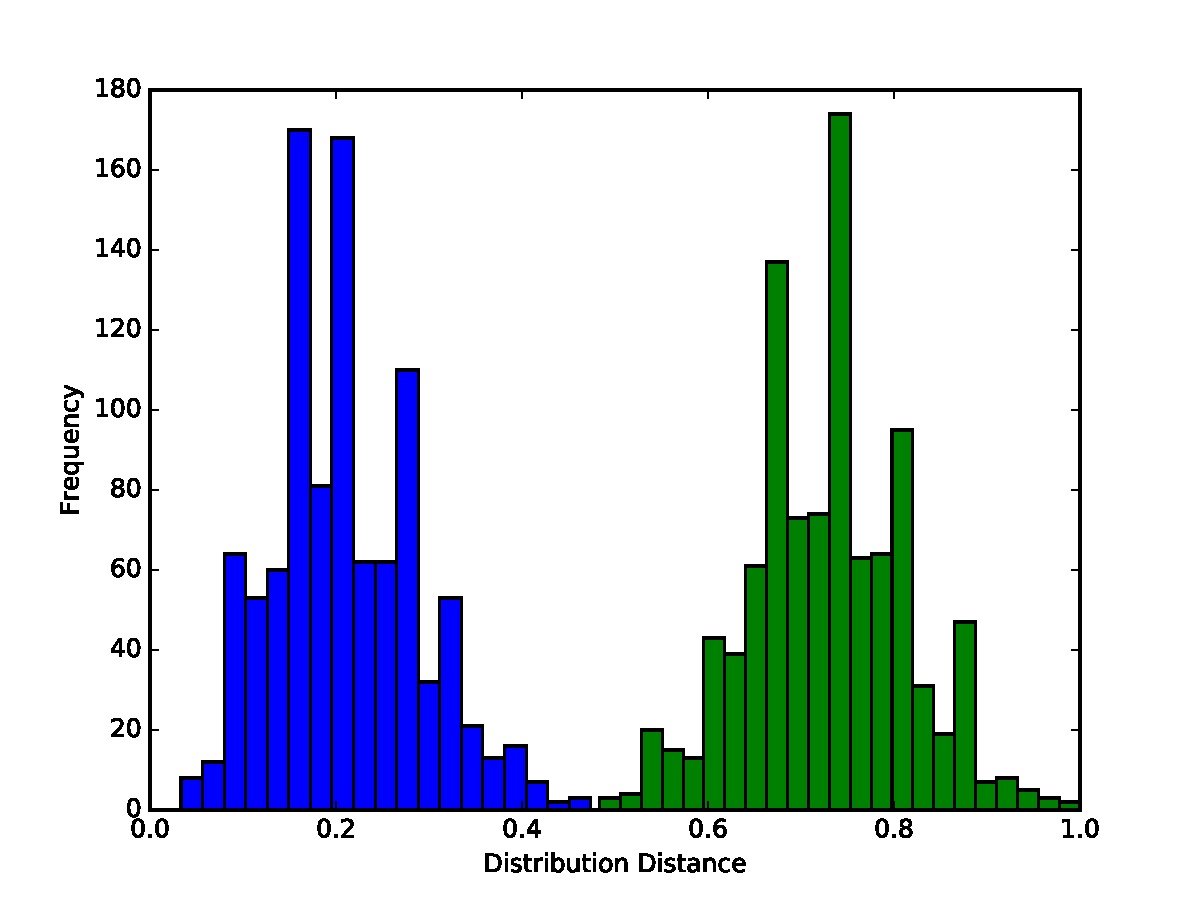
\includegraphics[scale=0.4]{profiler1.ps}
  \caption{Four classes overlapping}
  \label{fig:distributionDistance1}
\end{subfigure}%
\begin{subfigure}{.5\textwidth}
  \centering
  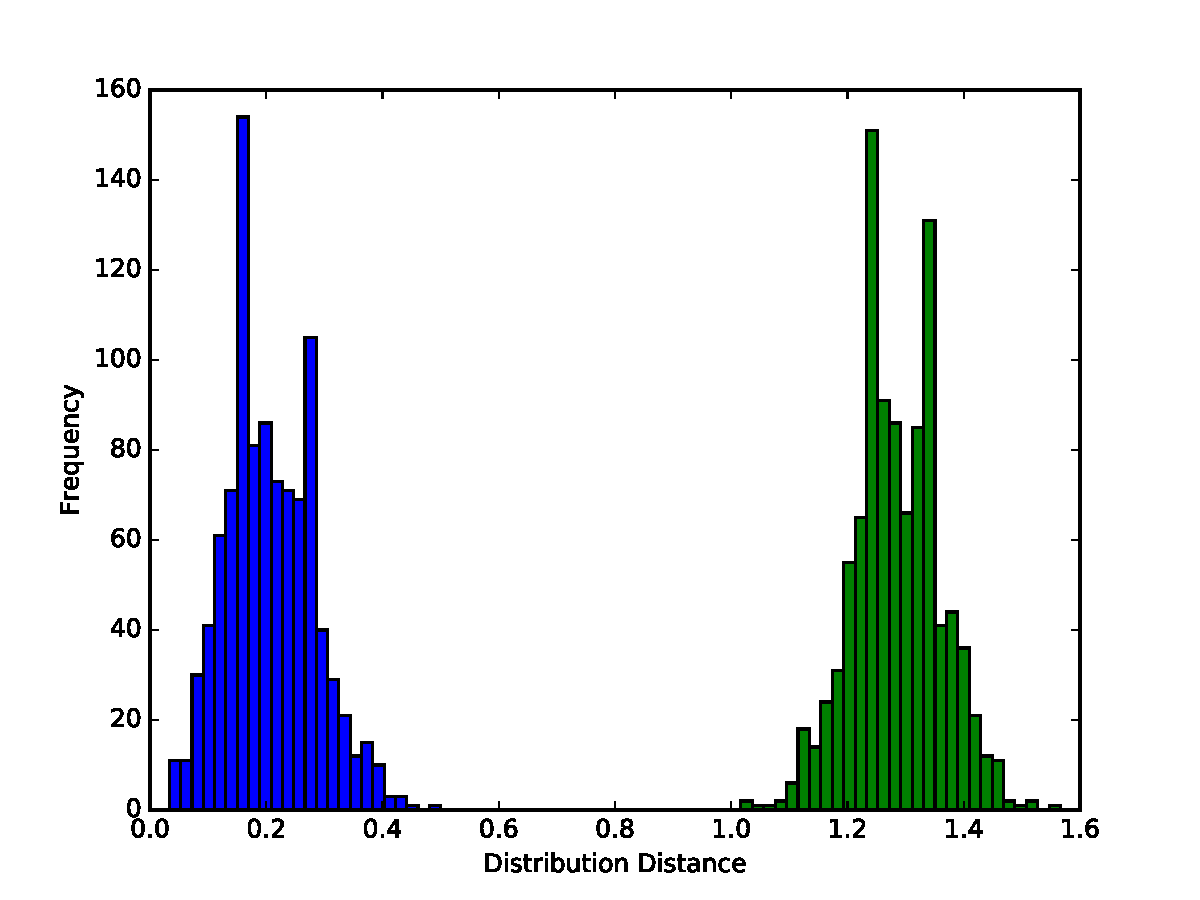
\includegraphics[scale=0.4]{profiler2.ps}
  \caption{Two classes overlapping}
  \label{fig:distributionDistance2}
\end{subfigure}

\caption{Graphs showing the distance between data distribution of two classes groups}
\label{fig:distributionDistance}
\end{figure*}



\section{Related Work}
\paragraph{Environment Information}

% Talk about the scenario
Many papers have talked about the difference between testing CNN models in the lab setting and in the wild. In lab setting, the prevalent benchmarks, like ImageNet \cite{deng2009imagenet} and CIFAR100 \cite{krizhevsky2009learning}, all assumes equal number of images for each class. However, in a more realistic setting \cite{han2016mcdnn, shen2016fast}, different classes may have dramatically different frequency and the distribution may also change over time. The question we want to answer is that, given an environment with a number of classes and distribution, how to use this information? All of the existing works \cite{han2016mcdnn, shen2016fast} only use transfer learning to retrain the last few layers, which would introduce a huge amount of energy consumption and time latency. Our method will make use of the distribution efficiently without finetuning, thus avoid additional energy-consumption and time latency.

% Unbalanced dataset
\paragraph{Unbalanced dataset}
Unbalanced datasets focus on the problem that training dataset has different distribution with the testing dataset, which is related to our scenario. One key point of the unbalanced dataset is that the minor classes in the training dataset cannot gain same attention as the major classes, thus oversampling on minor classes or undersampling on major classes will be implemented to generate a balanced dataset \cite{hoens2012learning, van2007experimental, wang2016dealing}. Our scenario is different since we assume that we have a model pretrained on a balanced dataset and in the testing time the class distribution changes. Another key point of the unbalanced dataset is that in the running time, as the distribution changes, the model will keep updating as new inputs come and finetuning is constantly needed. Our method avoids retrain at all and could achieve the same or better performance by only changing a few parameters according to the distribution automatically. Thus energy efficiency and speedup could be achieved by our solution.


% Talk about transfer learning
\paragraph{Transfer learning}
Transfer learning has shown benefit in domain adaption and currently is the dominant method, if not the only one, for domain adaption. To solve the problem that the testing dataset is small, we use transfer learning \cite{oquab2014learning}. To use unsupervised dataset \cite{doersch2015unsupervised, noroozi2016unsupervised}, we use transfer learning. Assume we have a large model handling $1000$ classes and in an environment where only $10$ classes appearing, we still use transfer learning \cite{han2016mcdnn, shen2016fast}. Transfer learning has become the only method off the top of the head when we consider the change in classes. Although transfer learning shows various benefit, it also has intrinsic shortage residing in the process of training a CNN model. First, it is hard to decide how many layers we should freeze. Published papers \cite{yosinski2014transferable} reported that freezing fewer layers leads to better performance on different domains and freezing more layers lead to a better performance on similar domains since the co-adapted interactions between layers will be kept. However, it is still hard to decide whether two domains are similar enough and the exact effect of freezing a various number of layers. Second, it is hard to decide the hyper-parameters unless actually trying different settings. When choosing epoch numbers, it is hard to predict whether the model will converge or collapse after a pre-chosen number of epochs. The choice of learning rate also depends on both model and dataset. The choice of hyper-parameter needs expertise in finetuning, which is lacked by the automatical product. Third, the long latency and energy consumption of training a model obstacle the transfer learning on energy-efficient devices, especially in an environment that class number and distributions keep changing. Our method can avoid retraining at all while adapting to the new dataset, thus all the inconvenience related to retraining is avoided naturally.

\paragraph{Distillation}
Distillation has been discussed extensively in machine learning area \cite{hinton2015distilling, ba2014deep, dauphin2013big, chen2017learning, lopez2015unifying, kim2015compression,bucilu2006model}. With distillation, we can use a smaller model to learn a complex model, get a better performance than the small model, and consume less energy than the complex model. Thus distillation naturally fits great with energy-efficiency on mobile device. However, neither the distillation people nor the mobile energy efficiency people considered combining these two techniques together. We are the first to introduce distillation into mobile energy efficiency. We solved obstacles in both side. First, existing distillation methods could only learn a large model when there are equal number of nodes in the softmax layer while our method could proceed no matter the difference between these two numbers. Second, existing papers could either only retrain last few layers \cite{li2015towards}, which lose the ability to change model architecture, or retrain the model from scratch \cite{han2016mcdnn, kang2017noscope, shen2016fast}, which lose the information contained in large model. Introducing distillation into runtime optimization can solve these problems perfectly.

\paragraph{Specialization}
Use specialization to generate a series of models composing trade-off between accuracy and energy is an emerging method for solving energy efficiency problem on mobile devices \cite{han2016mcdnn, kang2017noscope, shen2016fast}. Generally the reduction in energy is achieved by reducing number of layers and the resulting decrease in accuracy is made up by reducing number of nodes in the softmax layer. Although existing papers introduced a new way to solve the energy efficiency problem, the implementation detail is very coarse-grained and there are lots of open questions to be answered. Instead of only considering number of classes in the runtime, our paper took class correlation into consideration and introduced semantic tree as a quantitative method describing similarity between classes. Based on the numeric metric, we brought up guided search to replace exhaustive search used in existing papers. The second contribution is to introduce distillation and varying input size into runtime optimization. Previously, the only method employed in this area is to reducing number of layers. We found that input size is also a simple but effective in specialization. Finally, \textit{probability layer} was proposed to act as cold-start, solved the time latency introduced by retraining, and gives more choice for the scheduling model.

\paragraph{Model compression}
Model compression is to compress CNN architecture through matrix factorization and matrix pruning. Matrix factorization \cite{jaderberg2014speeding, kim2015compression, romero2014fitnets, xue2014singular} means using the multiplication of two low rank matrices to replace a single high rank matrix. Matrix pruning \cite{chen2015compressing, han2015learning} is to transform a matrix into sparse matrix by pruning small digits to be zero. Both directions of model compression do not change the number of nodes in the softmax layer or the model architecture. Thus techniques in model compression is orthogonal to using runtime distribution and could provide further optimization after reducing number of classes. 


\paragraph{Early stop}
Early stop \cite{teerapittayanon2016branchynet, panda2016conditional} is an architecture with branches and will stop calculating once a branch is enough confident that an image has been classified correctly. Early stop contains various architectures to achieve energy efficiency through reducing unnecessary computation. This is orthogonal to runtime specialization and could be included into the model bank.

\section{Conclusion and Future Work}
We have presented probability layer which exploits runtime environment information to increase prediction accuracy. Probability layer requires only a single extra layer after the general CNN models with unnoticeable extra computation and obtains a boost in accuracy. Compared to transfer learning, probability layer achieves comparable or even better accuracy boost, avoids retraining, and maintain the ability to detect new classes. Additionally, probability layer can be combined with acceleration methods which exploit various types of network redundancy to achieve further speedups.




\bibliography{references}
\bibliographystyle{plain}


\end{document}

